\documentclass[aspectratio=169]{beamer}

% \usepackage{mypresentationstyle}
% \usepackage{multicol}
% \usepackage{biblatex}

%\usepackage{svg}

\newcommand{\tlapack}{{$\langle$T$\rangle$LAPACK}}

\newcommand{\gitmerged}{
\includegraphics[height=1em]{screenshots/git-merged.png}}
%\newcommand{\gitmerged}{
\includegraphics[height=1em]{screenshots/Octicons-git-merge.svg.png}}
\newcommand{\gitPR}{
\includegraphics[height=1em]{screenshots/Octicons-git-pull-request.svg.png}}


\title{Building momentum for a community-based (dense) BLAS evolution}
\author{Julien Langou}
\date{25 March 2026}
\usetheme{Copenhagen}
%\addbibresource{references.bib}
\begin{document}
\begin{frame}
\titlepage
\end{frame}
% \begin{frame}{Table of Contents}
% \tableofcontents
% \end{frame}
% \section{Computing the Q Factor}
\begin{frame}{History}

\begin{itemize}
\item[\pgfuseimage{beamericonarticle}]
C. L. Lawson, R. J. Hanson, D. R. Kincaid, and F. T. Krogh.
Basic Linear Algebra Subprograms for Fortran usage.
ACM Trans. on Math. Software 5, 3 (Sept. 1979) 308–323.
\item[\pgfuseimage{beamericonarticle}]
J. J. Dongarra, J. Du Croz, S. Hammarling, and R. J. Hanson.
An extended set of FORTRAN Basic Linear Algebra Subprograms.
ACM Trans. on Math. Software 14, 1 (March 1988) 1–17.
\item[\pgfuseimage{beamericonarticle}]
J. J. Dongarra, J. Du Croz, S. Hammarling, and I. Duff.
A set of level 3 Basic Linear Algebra Subprograms.
ACM Trans. on Math. Software 16, 1 (March 1990) 1–17.
\end{itemize}

Points:
\begin{itemize}
\item enable portable performance
\item paradigm for LAPACK design (and other applications, e.g. AI nowadays)
\item low surface / volume ratio for Level 3 BLAS
\end{itemize}

\end{frame}

\begin{frame}{BLAST Forum}

\pgfuseimage{beamericonarticle}~L. Susan Blackford, James Demmel, Jack Dongarra, Iain Duff, Sven Hammarling, Greg Henry, Michael Heroux, Linda Kaufman, Andrew Lumsdaine, Antoine Petitet, Roldan Pozo, Karin Remington, and R. Clint Whaley.
An updated set of basic linear algebra subprograms (BLAS). ACM Trans. Math. Softw. 28, 2 (June 2002), 135–151. 
\url{https://doi.org/10.1145/567806.567807}

%January 23, 2001.
%\url{https://www.netlib.org/blas/blast-forum/}

%An Updated Set of Basic Linear Algebra Subprograms (BLAS)
%\url{https://www.netlib.org/blas/blast-forum/blaspaper1.pdf}

Led to XBLAS, Sparse BLAS, etc.

\end{frame}


\begin{frame}{Other efforts}

\pgfuseimage{beamericonarticle}~RandBLAS\\
\url{https://randblas.readthedocs.io/en/1.1.0/}

\pgfuseimage{beamericonarticle}~SparseBLAS\\
\url{https://arxiv.org/abs/2411.13259}

\end{frame}


\begin{frame}{Adding to the BLAS (1/3)}

\begin{itemize}
\item Complex ecosystem with a reference implementation and optimized implementations
%\begin{itemize}
%\item FlexiBLAS, OpenBLAS, BLIS, 
%\item MKL, AOCL, Accelerate, 
%\end{itemize}
\item Inertia
\item Antiquated software architecture
\item scdz, BLAS, CBLAS, 64-bit interfaces, documentation, build process
\item TRSM = $2 \times 2 \times 3 \times 2 = 24$ variants
\item initially well done 
\end{itemize}


\end{frame}

\begin{frame}{Adding to the BLAS (2/3)}

Pressing needs and libraries are not waiting. In the past IBM ESSL was a good
example, but nowadays, standard to have ``interesting'' functionality in
libraries and not in reference BLAS.\\

It would be good to get head (proactive) of needed changes/additions as opposed
to play cacth-up (reactive).\\

\underline{Note:} A quirk is that BLAS is packaged within LAPACK. This has some cons and some pros. 
BLAS release numbers are tied to LAPACK release numbers.\\

\underline{Note:} ``Adding'' to the BLAS, we do not speak about ``changing'' any interfaces.

\end{frame}

\begin{frame}{Adding to the BLAS (3/3)}

A process:
\begin{itemize}
\item high level: need, adoption, interface, reference implementation
\item scdz, BLAS, CBLAS, 64-bit interfaces, build process
\item test
\item documentation
\item use it in LAPACK
\item GitHub, pull request, community discussion, community review
\end{itemize}

\end{frame}


\begin{frame}{Creating new BLAS libraries}

Congratulations, you decided that you wanted to write a full grown BLAS library. 
How do you check your BLAS library for correctness?

\begin{itemize}

\item BLAS has a test suite

\item check your BLAS with the LAPACK test suite (that checks LAPACK
functionality but exercises your BLAS in many and ``surprising'' way).

\end{itemize}

Related question: does LAPACK uses the whole for BLAS? No. 
List of routines that are not used:
CSYMM,
CSYR2K,
CSYRK,
ZSYMM,
ZSYR2K,
ZSYRK,
DCABS1,
SCABS1,
DROTMG,
SROTMG,
DSDOT,
SDSDOT.



\end{frame}




\begin{frame}{recent updates (1/5) - NRM2 (1/2)}

%\href{https://github.com/Reference-LAPACK/lapack/pull/514}{PR-514}
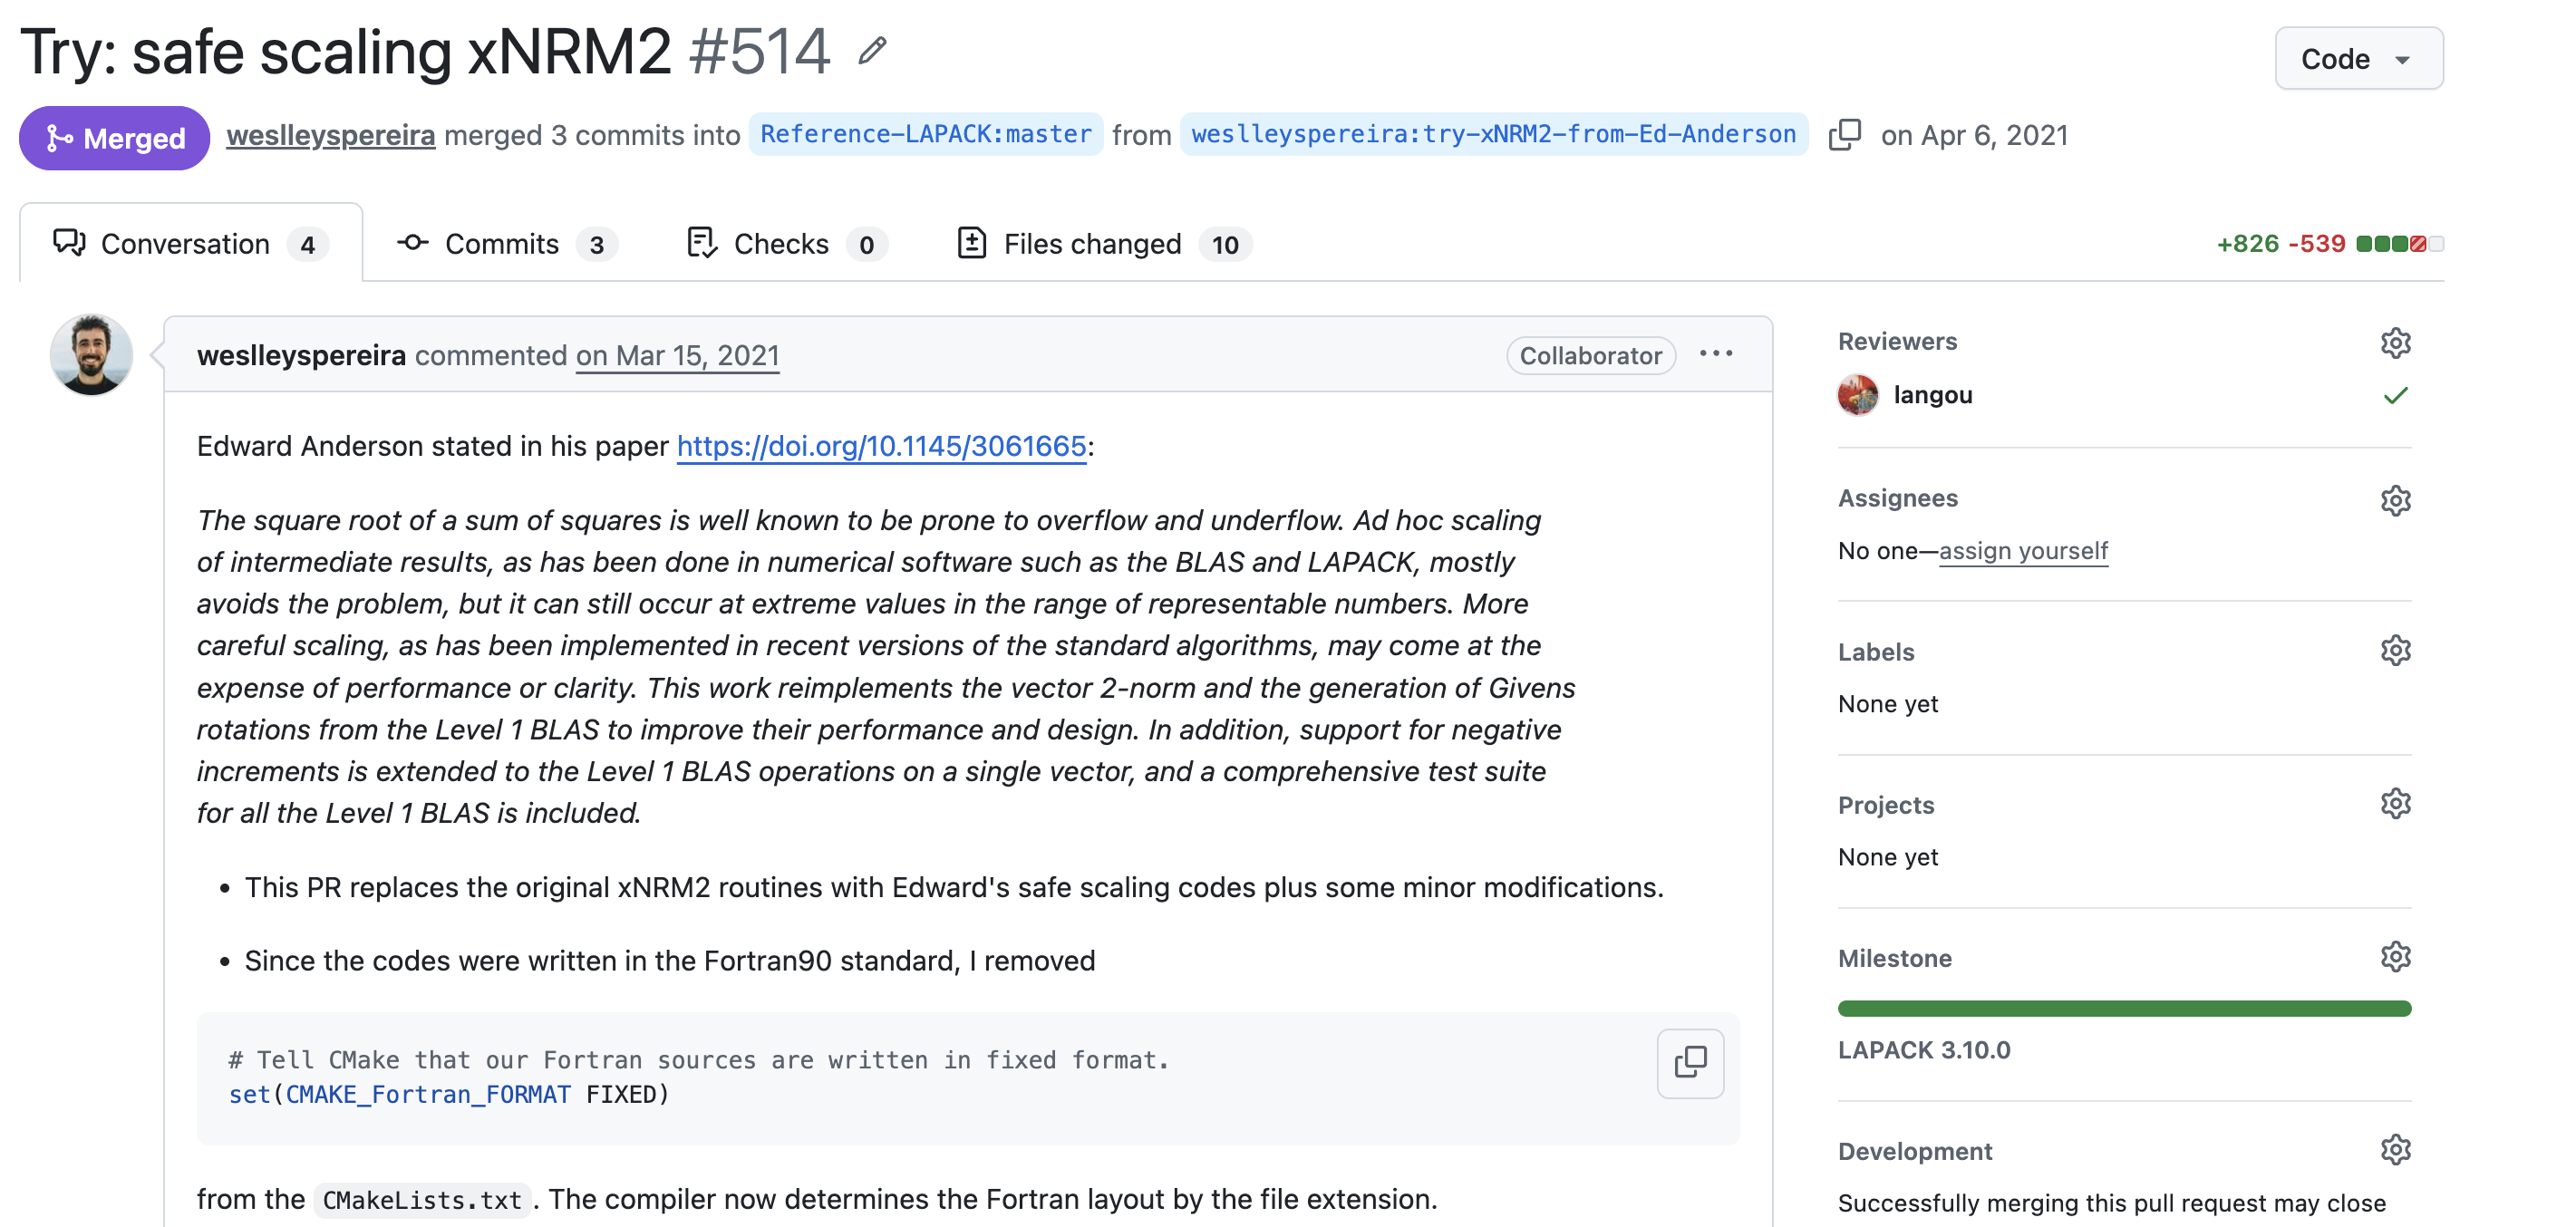
\includegraphics[width=\textwidth]{screenshots/ed-anderson-blue.png}

\end{frame}

\begin{frame}{recent updates (1/5) - NRM2 (2/2)}

\begin{itemize}
\item[\pgfuseimage{beamericonarticle}]
Anderson E. (2017).
Algorithm 978: Safe Scaling in the Level 1 BLAS.
ACM Trans Math Softw 44:1--28.
\url{https://doi.org/10.1145/3061665}
\item[\pgfuseimage{beamericonarticle}]
Blue, James L. (1978).
A Portable Fortran Program to Find the Euclidean Norm of a Vector.
ACM Trans Math Softw 4:15--23.
\url{https://doi.org/10.1145/355769.355771}
\end{itemize}

\end{frame}


\begin{frame}{recent updates (2/5) - ICAMAX}

%\href{https://github.com/Reference-LAPACK/lapack/pull/1116}{PR-1116}
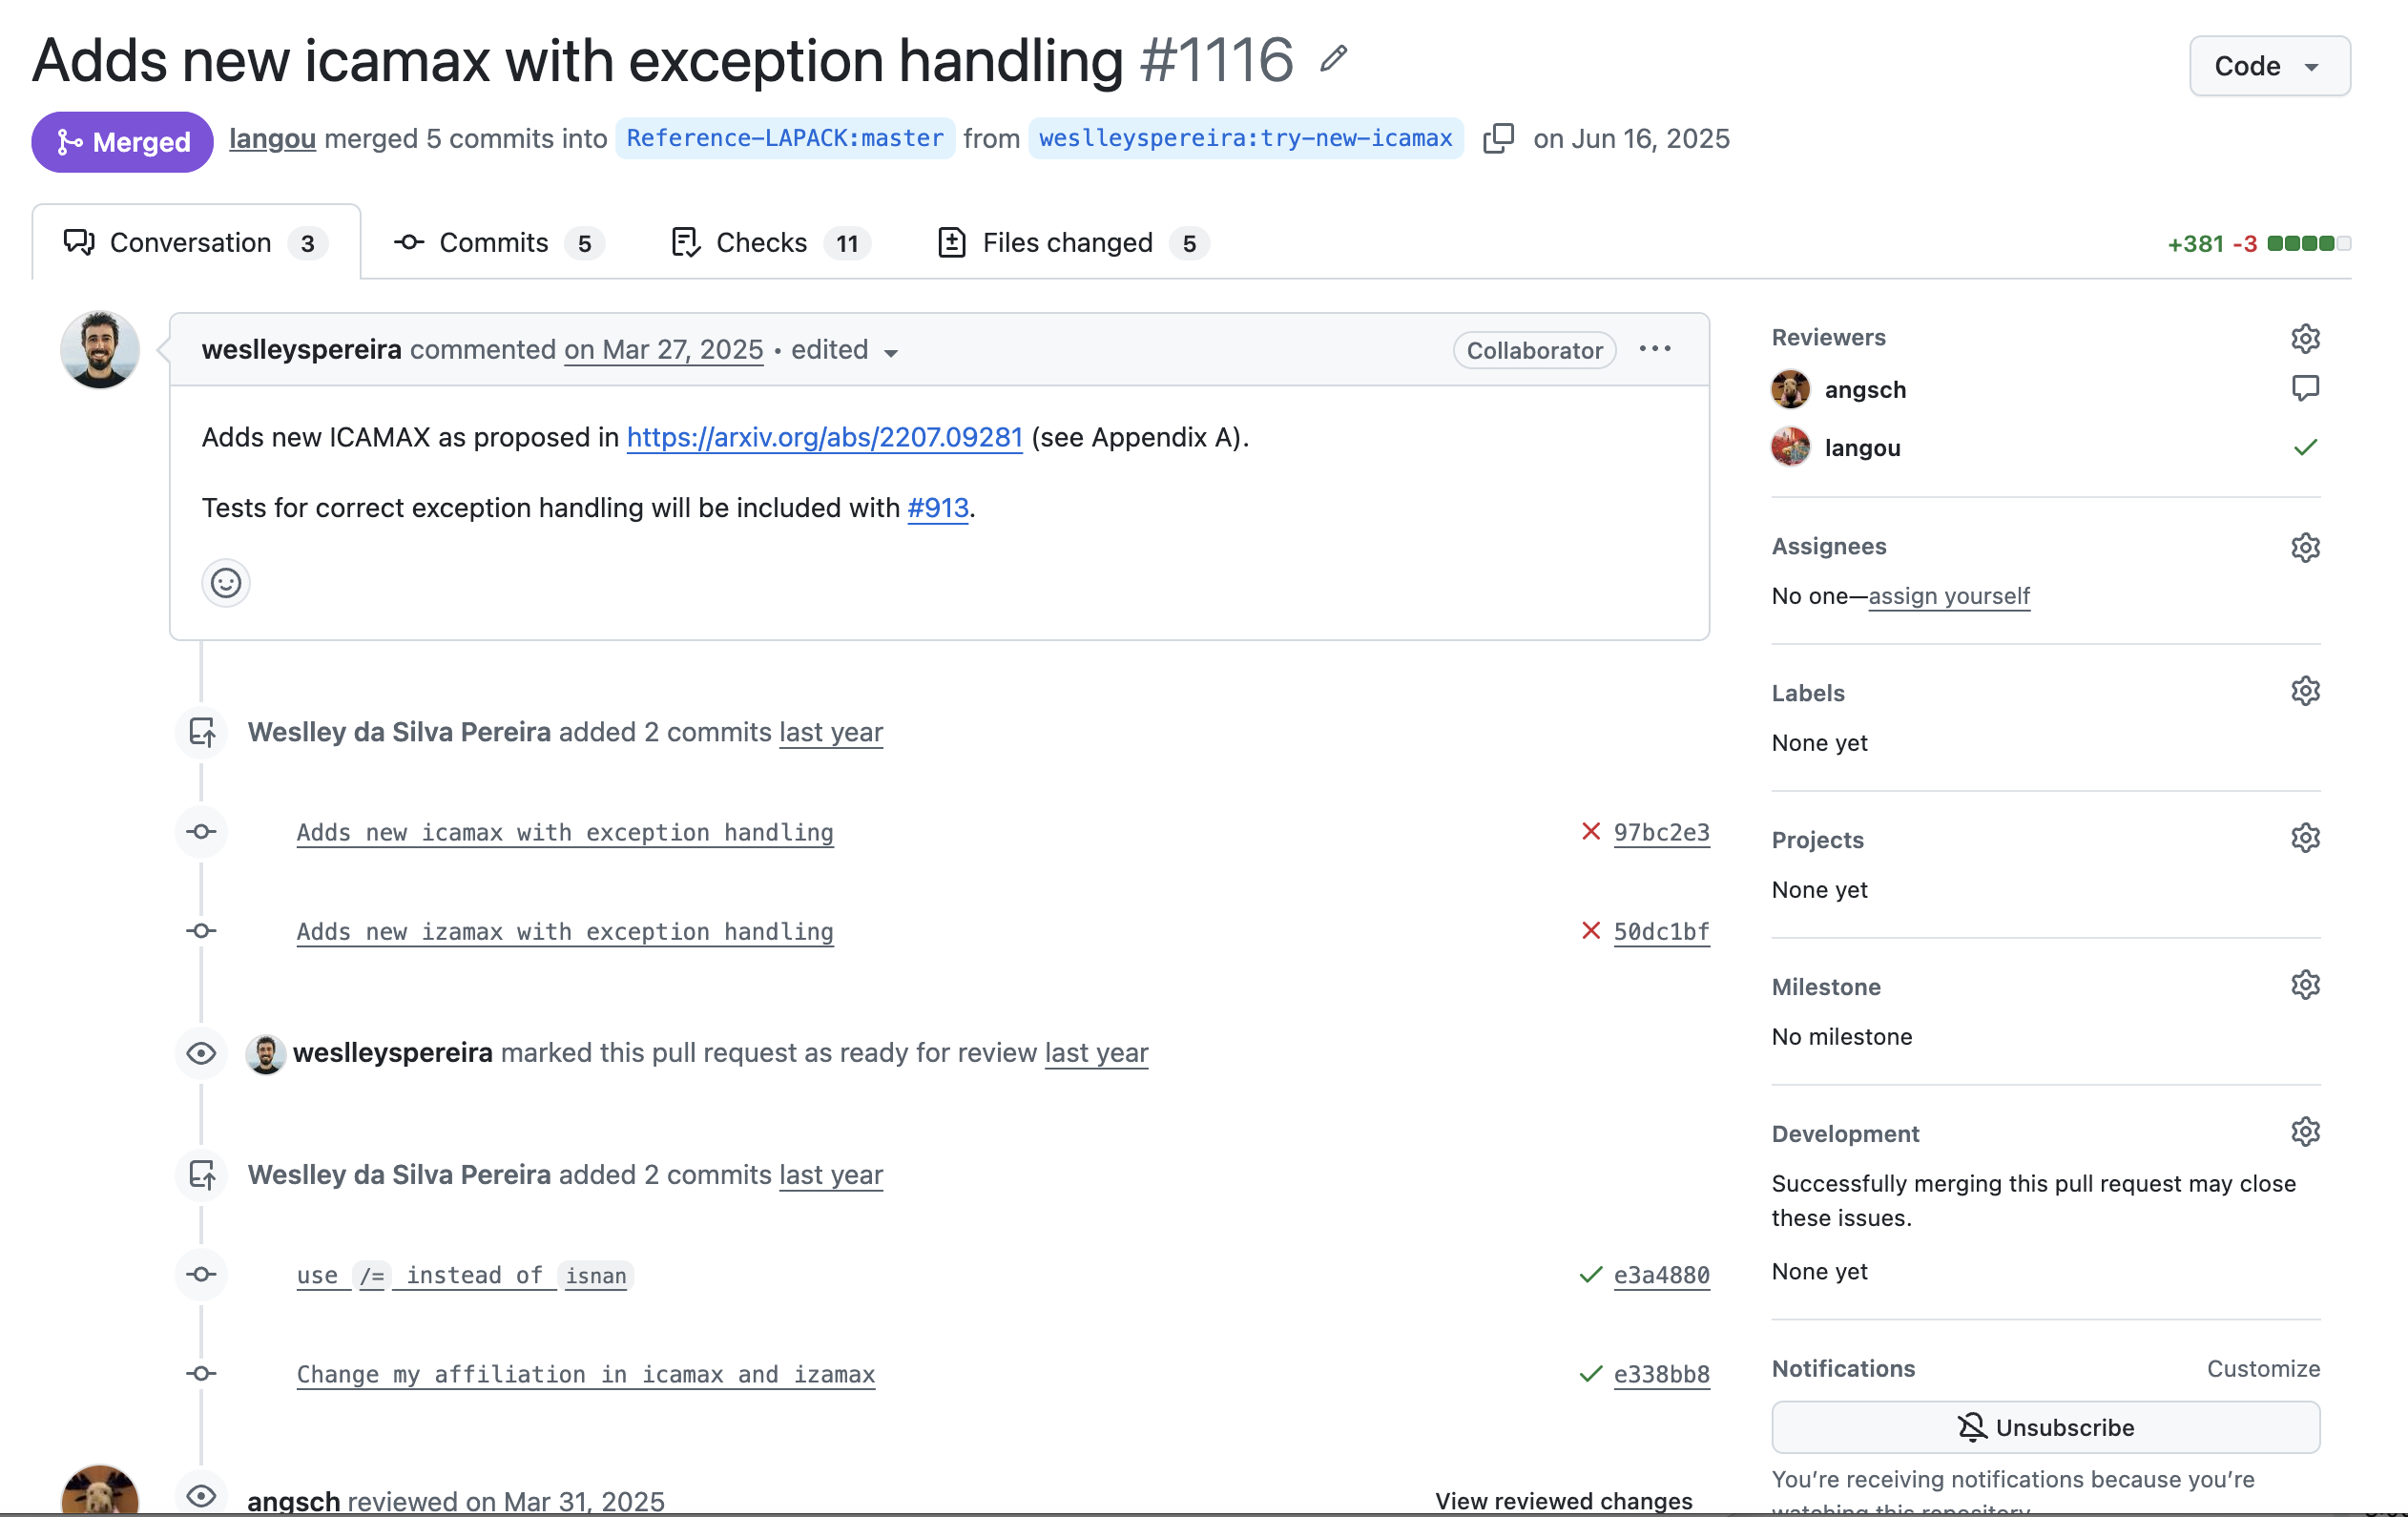
\includegraphics[width=\textwidth]{screenshots/ICAMAX.png}

\end{frame}



\begin{frame}{recent updates (3/5) - GEMMTR (1/2)}

%\href{https://github.com/Reference-LAPACK/lapack/pull/887}{\gitmerged PR-887}, Martin K{\"o}hler
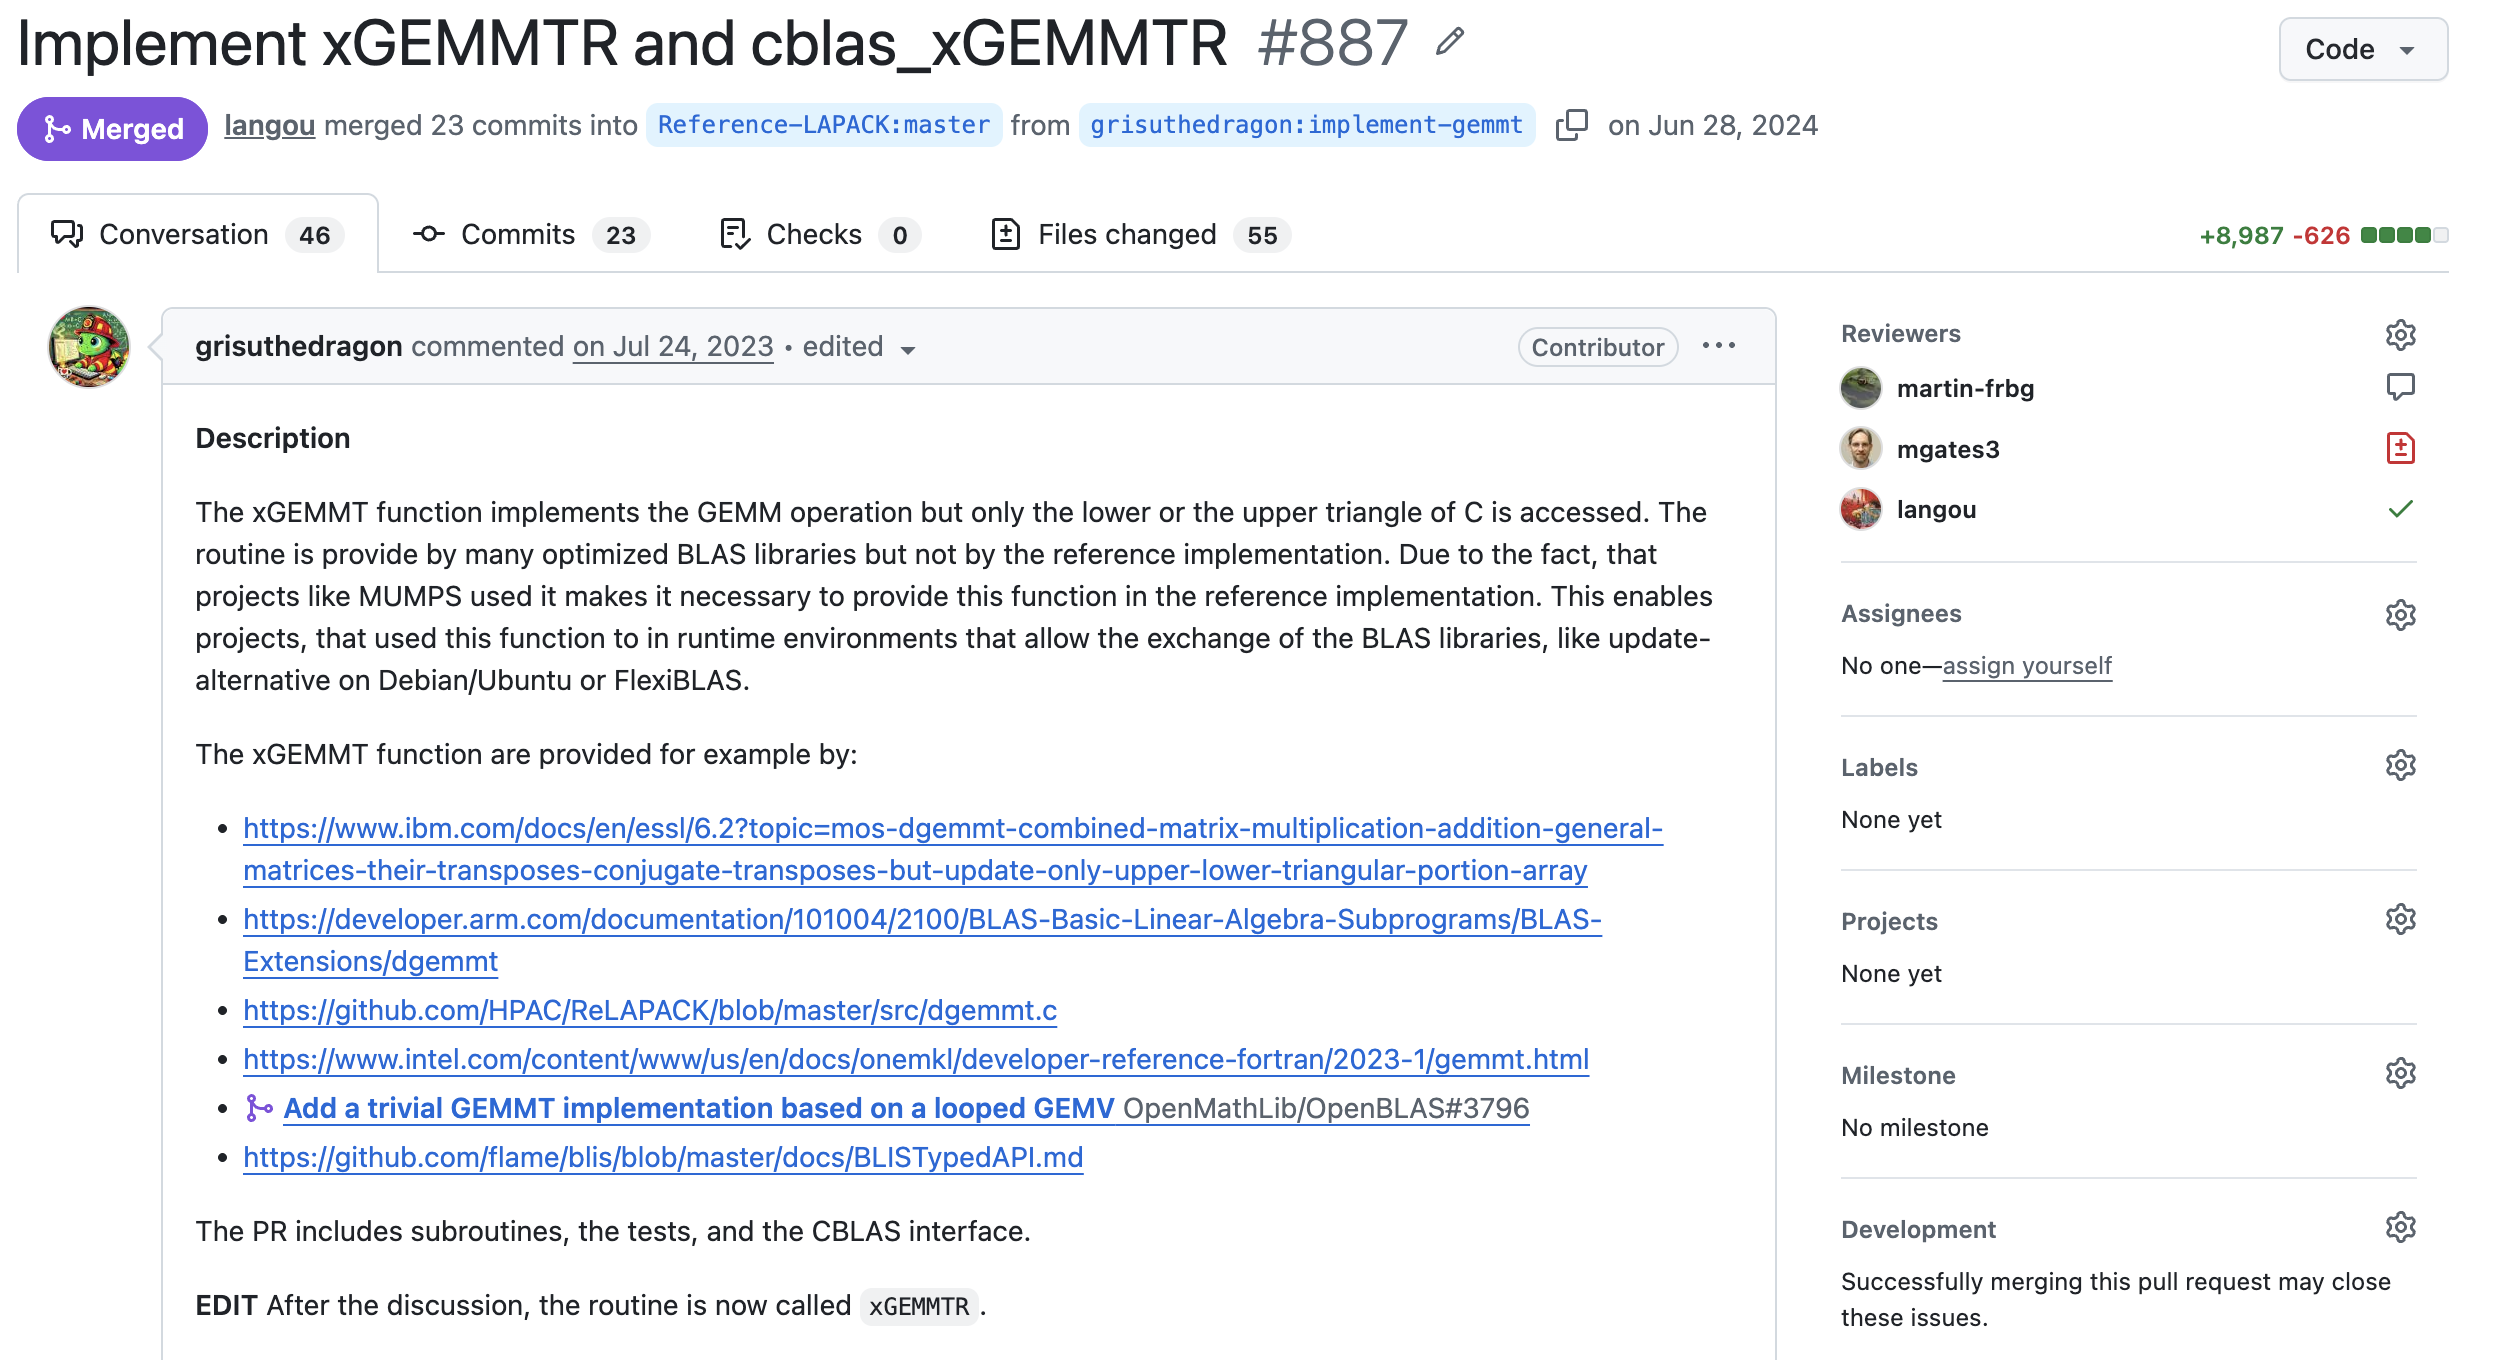
\includegraphics[width=\textwidth]{screenshots/GEMMTR-1.png}

\end{frame}

\begin{frame}{recent updates (3/5) - GEMMTR (2/2)}

%\href{https://github.com/Reference-LAPACK/lapack/pull/1069}{\gitmerged PR-1069}, Angelika Schwartz
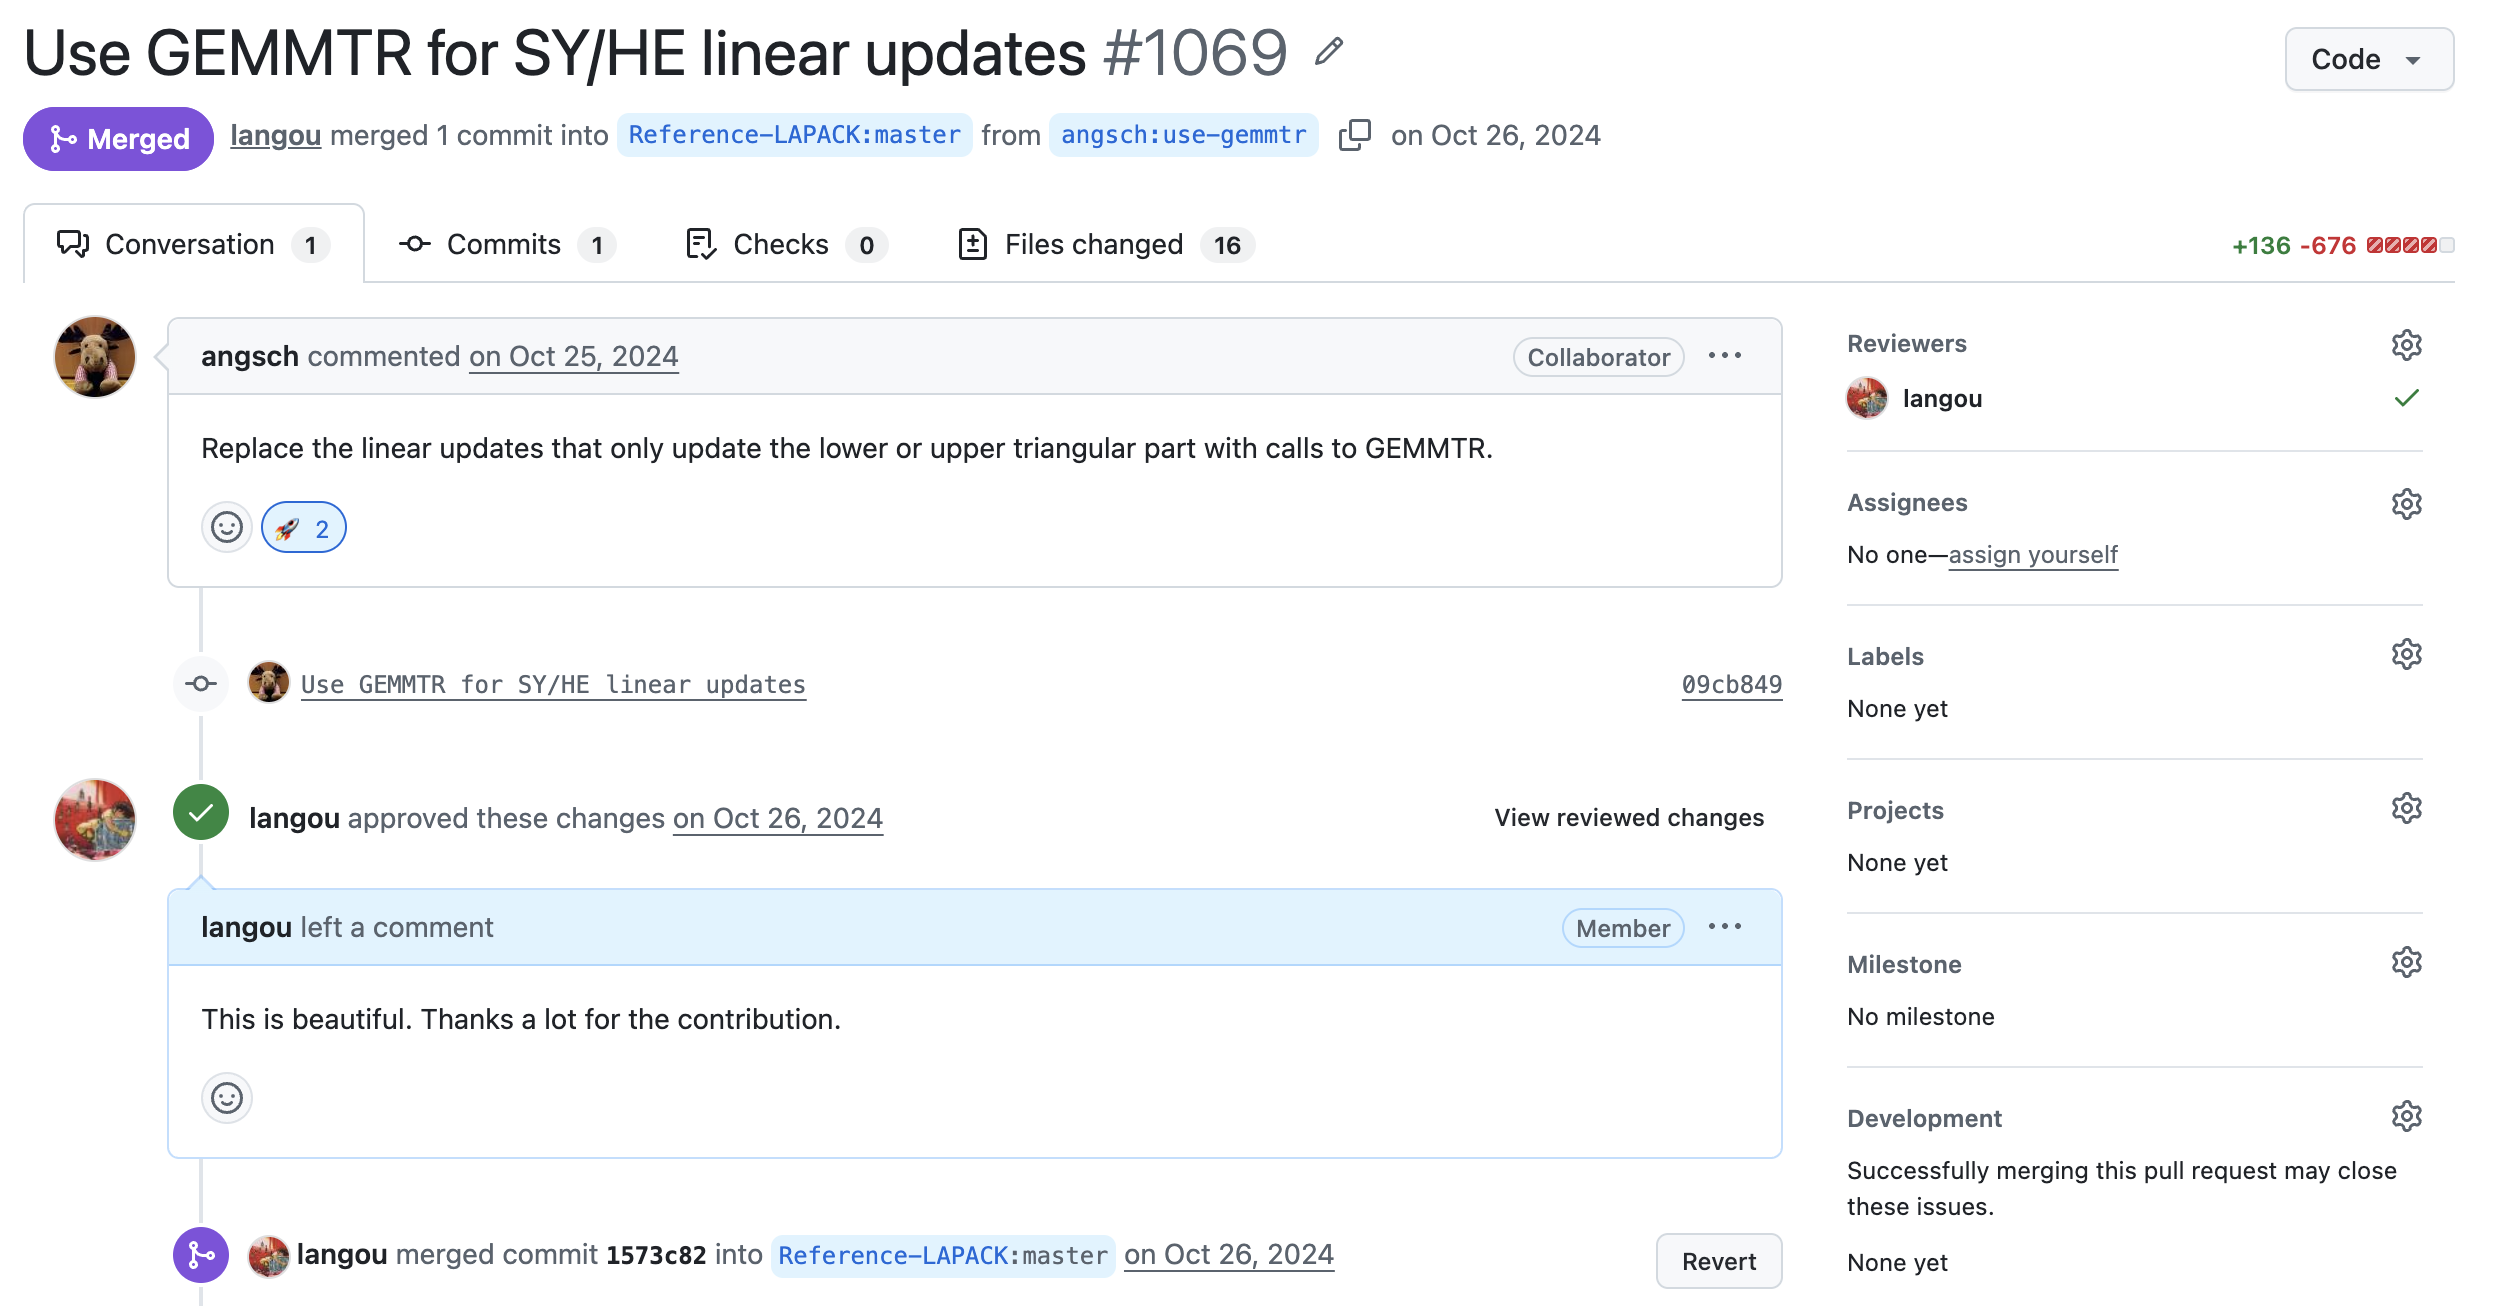
\includegraphics[width=\textwidth]{screenshots/GEMMTR-2.png}

\end{frame}

\begin{frame}{recent updates (4/5) - AXPBY}

%\href{https://github.com/Reference-LAPACK/lapack/pull/1048}{PR-1048}
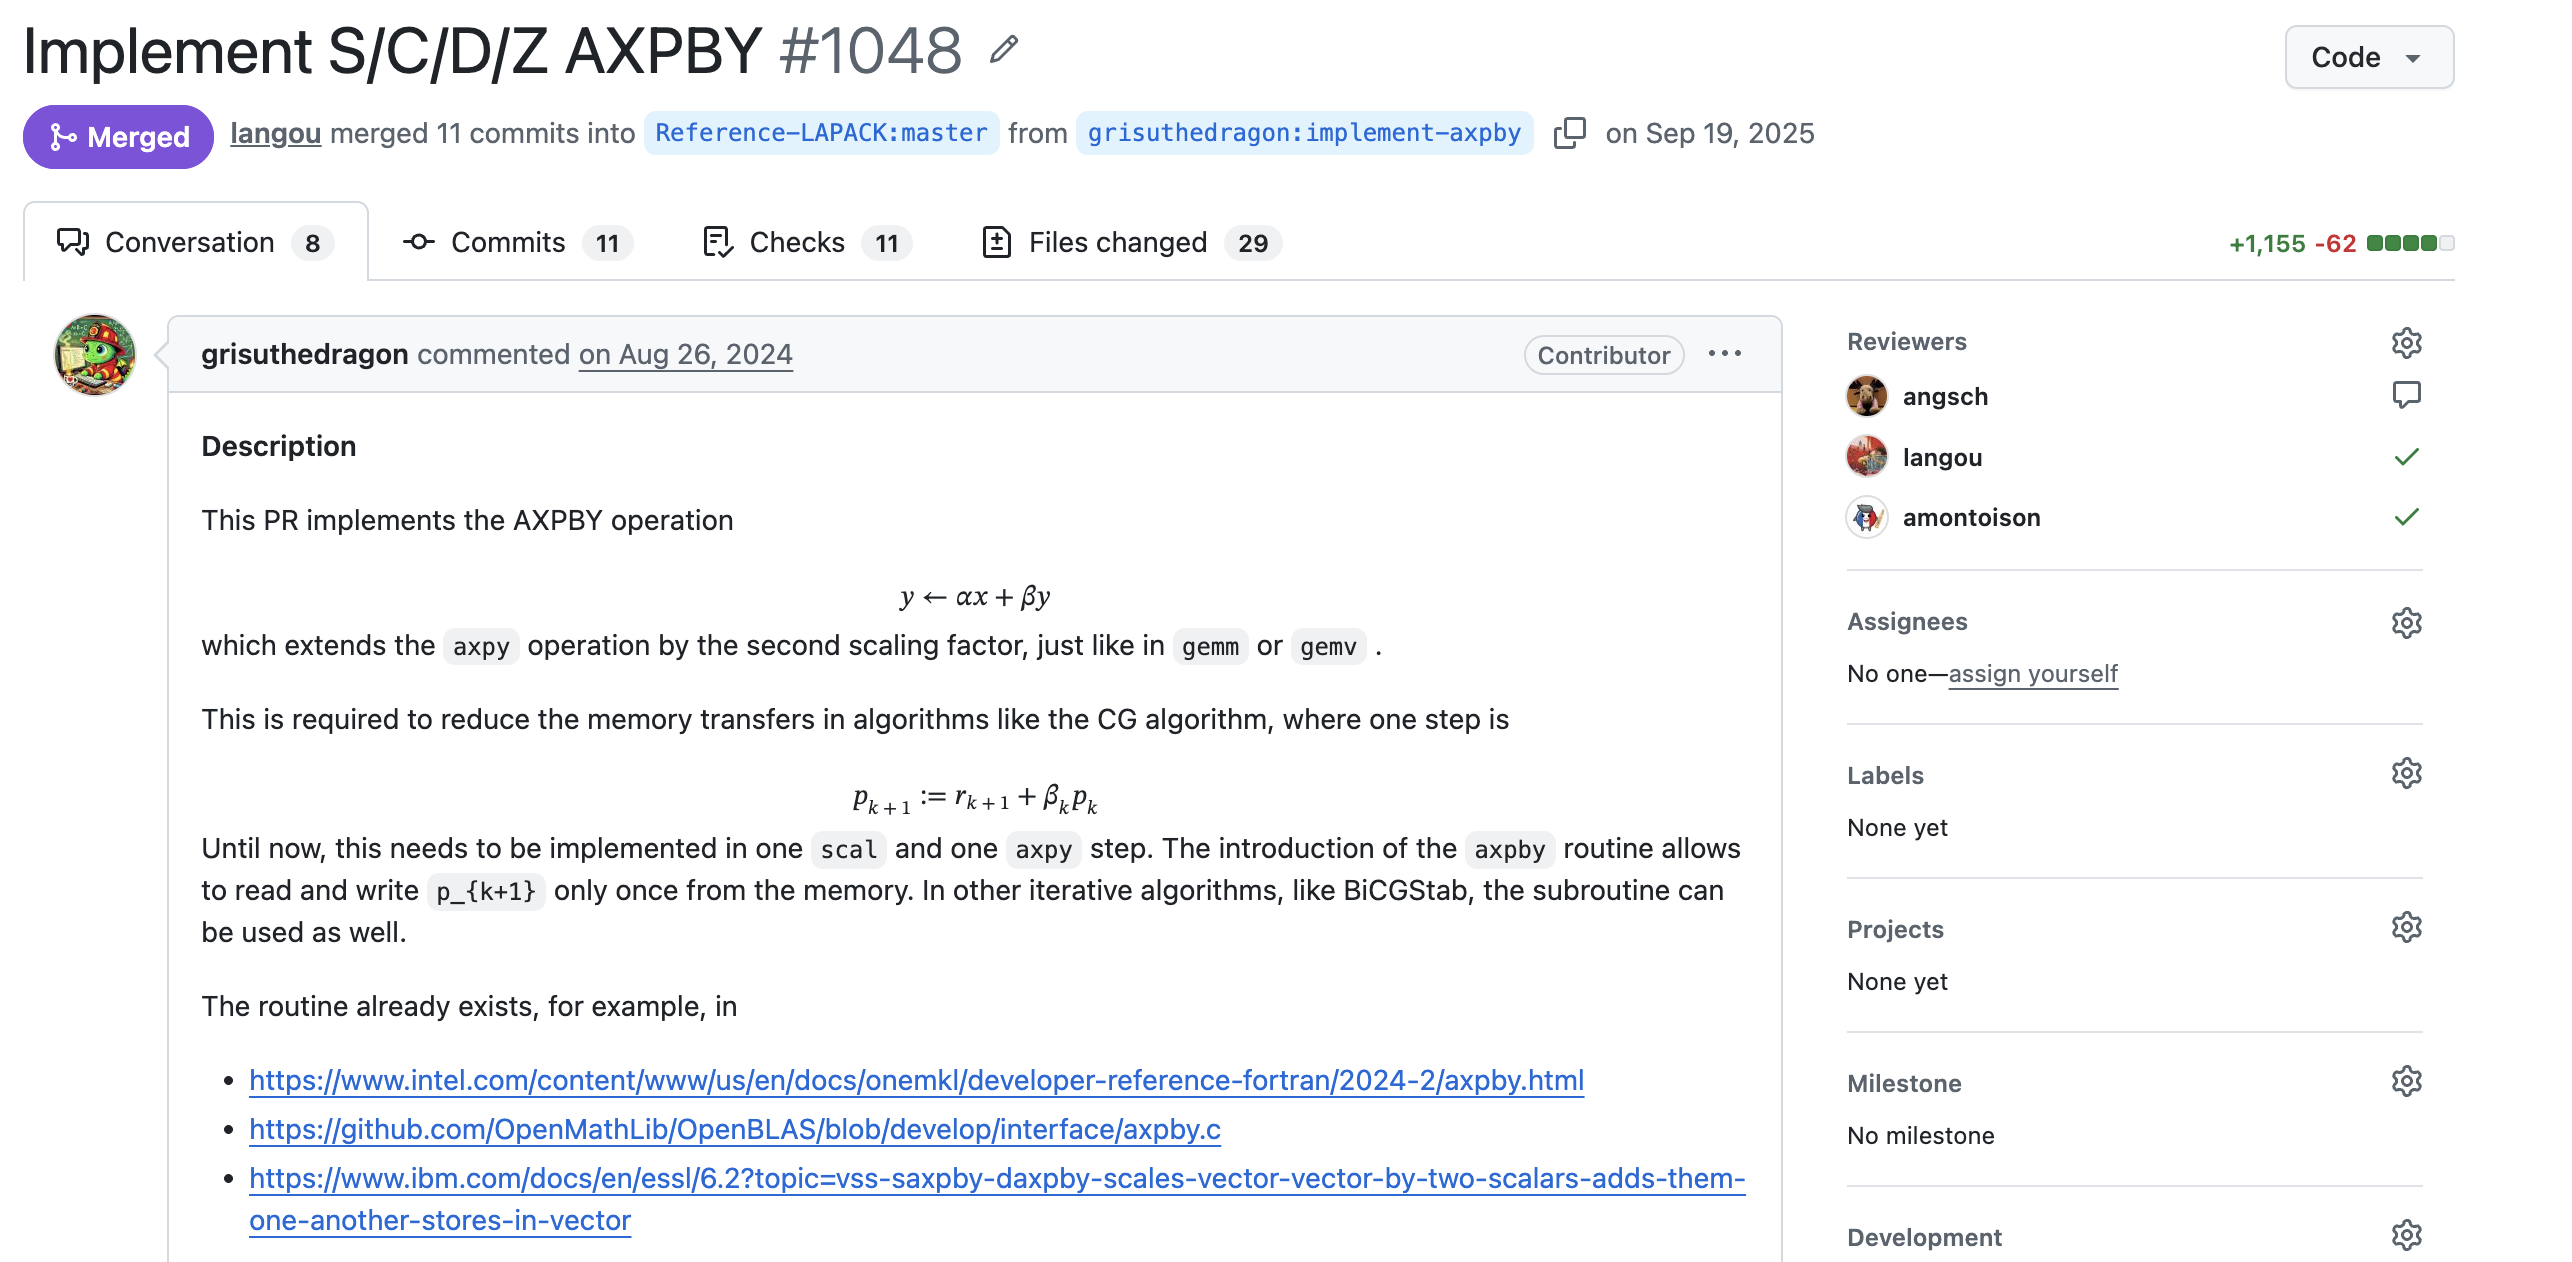
\includegraphics[width=\textwidth]{screenshots/AXPBY.png}

\end{frame}

\begin{frame}{recent updates (5/5) - sskewsymv}

%\href{https://github.com/Reference-LAPACK/lapack/pull/1116}{PR-1116}
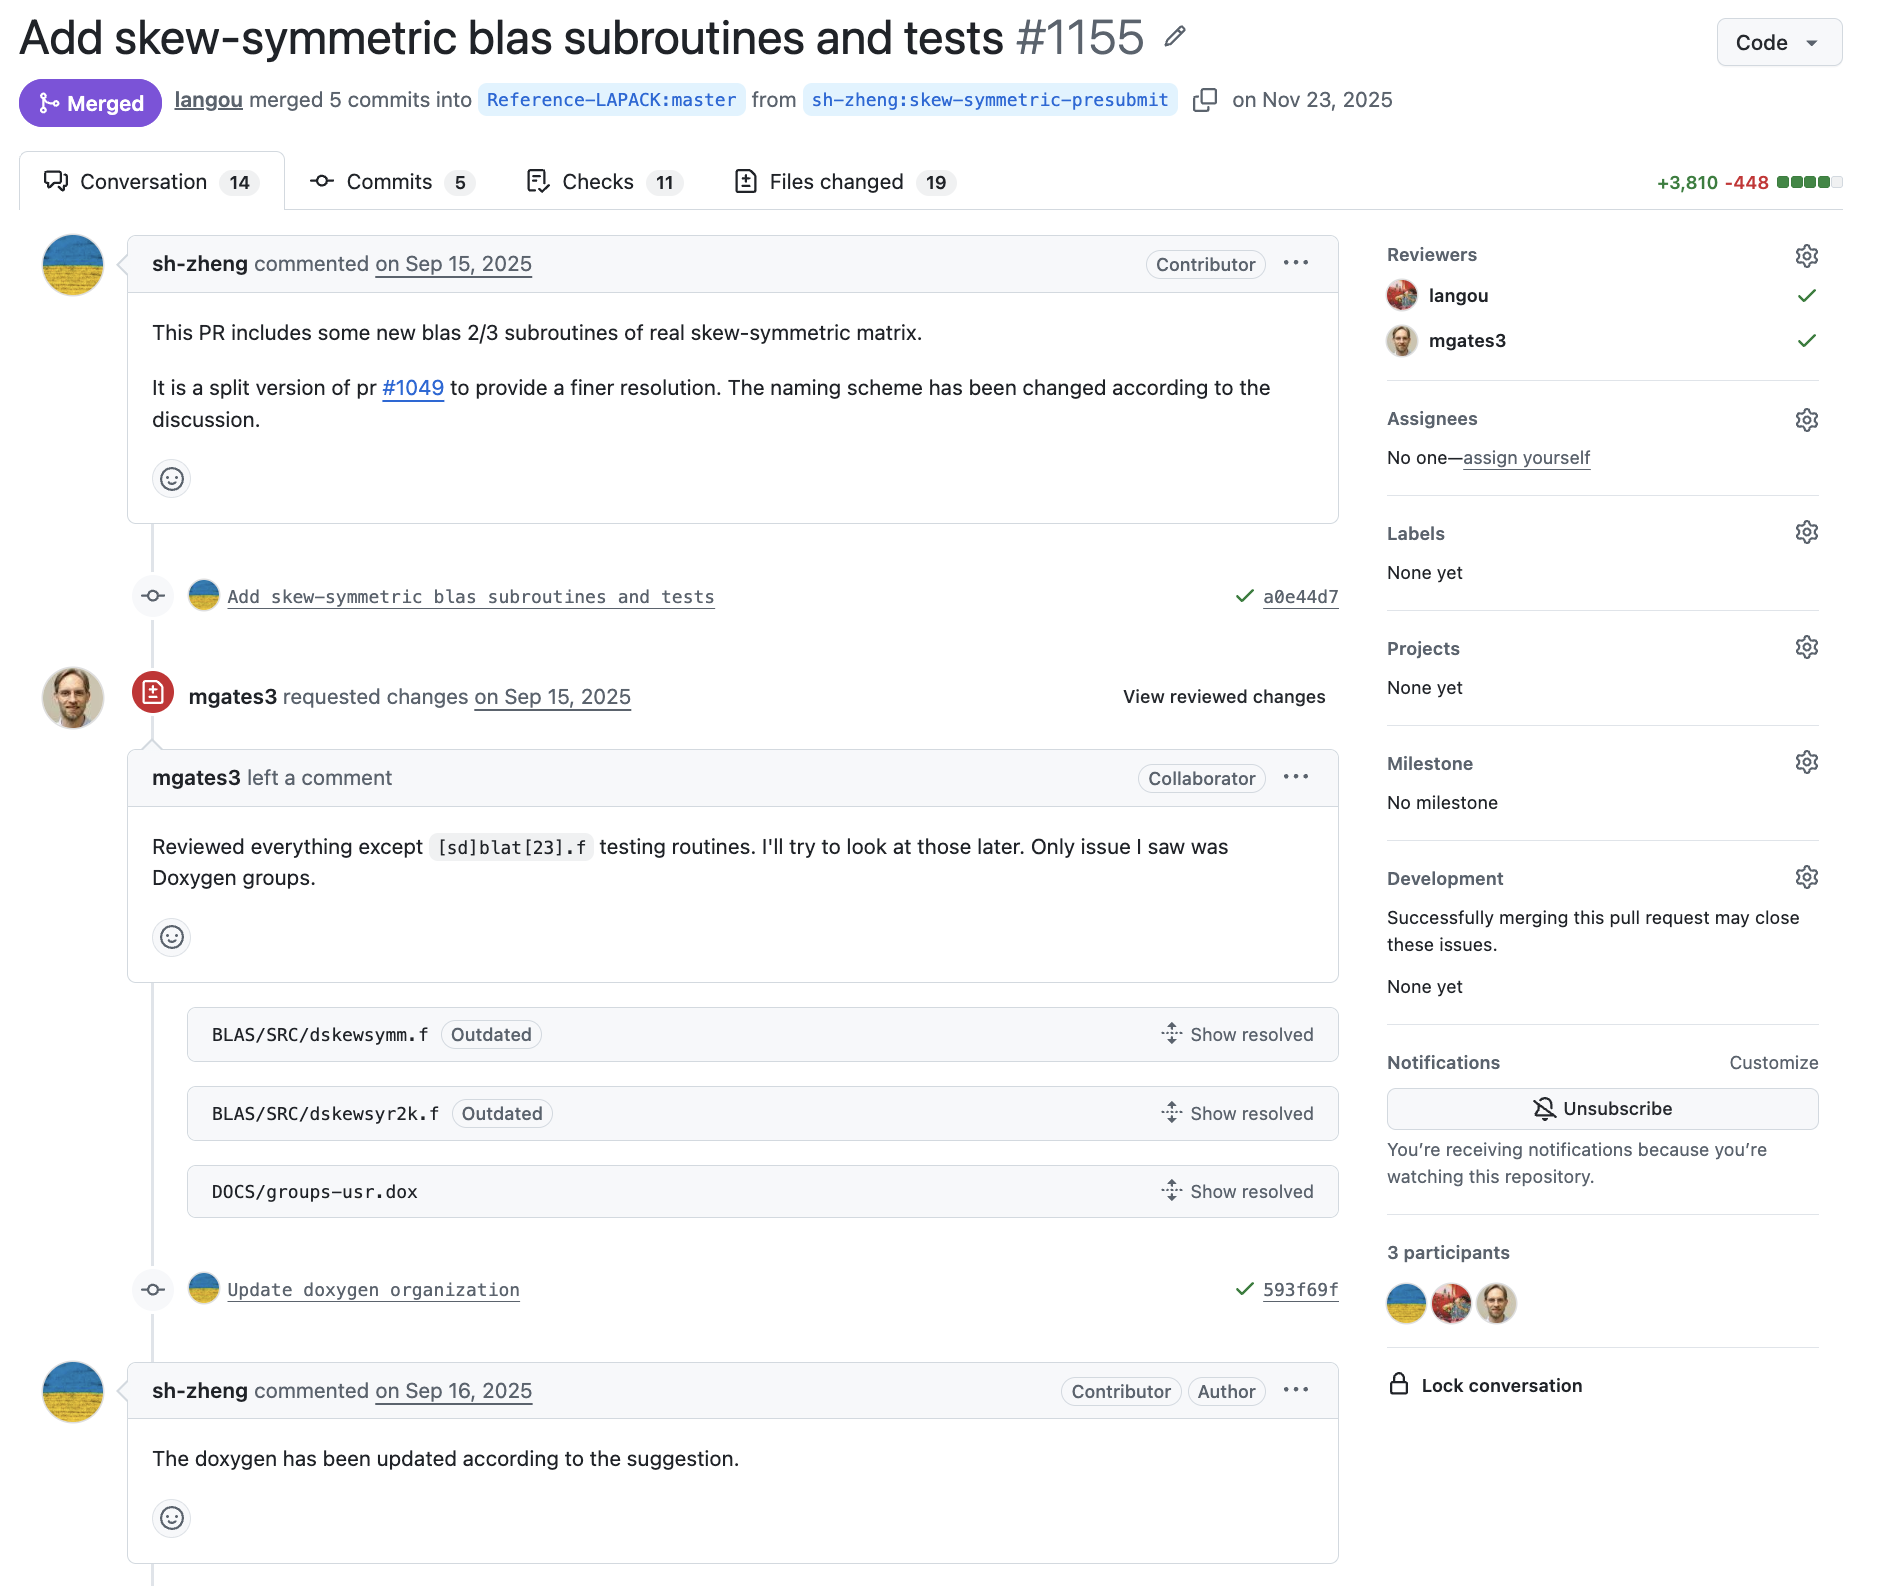
\includegraphics[width=\textwidth]{screenshots/SSKEWSYMV.png}

\end{frame}




\begin{frame}{work in progress / position paper (1/2) :: Consistent Exception Handling}

\pgfuseimage{beamericonarticle}~James Demmel, Jack Dongarra, Mark Gates, Greg Henry, Julien Langou, Xiaoye Li, Piotr Luszczek, Weslley Pereira, Jason Riedy, and Cindy Rubio-Gonz{\'a}lez. Proposed Consistent Exception Handling for the BLAS and LAPACK. 
2022 IEEE/ACM Sixth International Workshop on Software Correctness for HPC Applications (Correctness).
Year: 2022, Pages: 1-9
DOI Bookmark: 10.1109/Correctness56720.2022.00006

\end{frame}


\begin{frame}{work in progress / position paper (2/2) :: Grading the BLAS}

Multidimensional:
\begin{itemize}
\item accuracy (varies with $n$, depends on algorithm, etc)
\item corner cases (incx < 0, etc.)
\item proper exception handling
\item completeness
\item performance, energy
\end{itemize}

A better test suite would be nice. See efforts from Jackson Vanover, Weslley Pereira, and Mark Gates.

\end{frame}

\begin{frame}{NaN Check (ad hoc)}

%\href{https://github.com/Reference-LAPACK/lapack/pull/514}{PR-514}
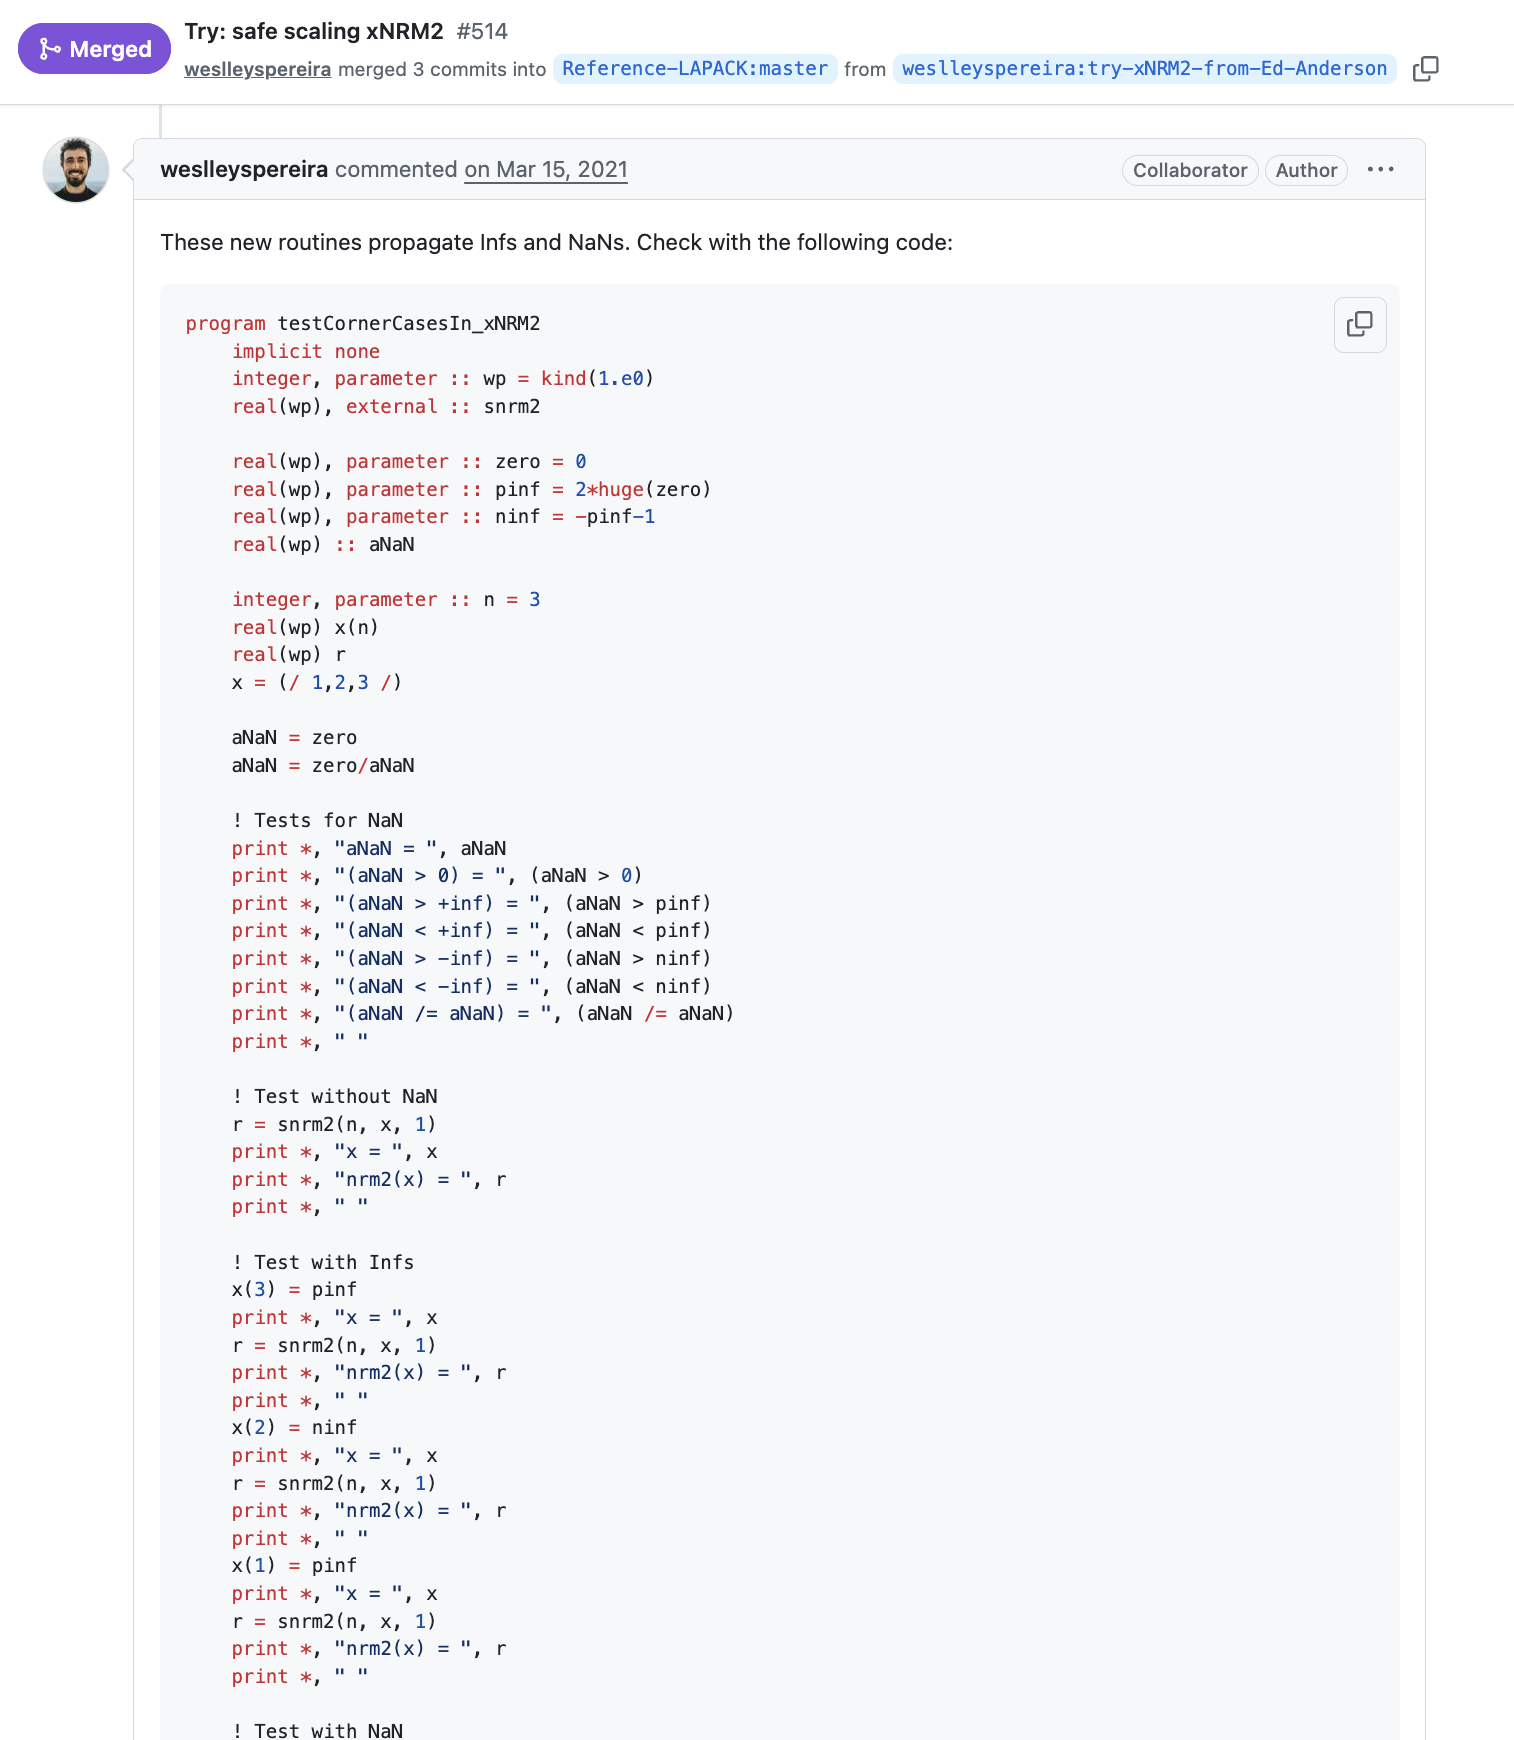
\includegraphics[width=\textwidth]{screenshots/NaNcheck.png}

\end{frame}


\begin{frame}{New possible developments}

\begin{itemize}
\item threading policy, execution policy%: there is multi-threaded BLAS but nothing really standard, 
\item mixed precisions
\item more precisions
\item more algorithms
\item batch BLAS
\item consistent exception handling
\end{itemize}

\end{frame}


\begin{frame}{accumulation in BLAS (1/3)}

%\href{https://github.com/Reference-LAPACK/lapack/issues/1180}{1180}
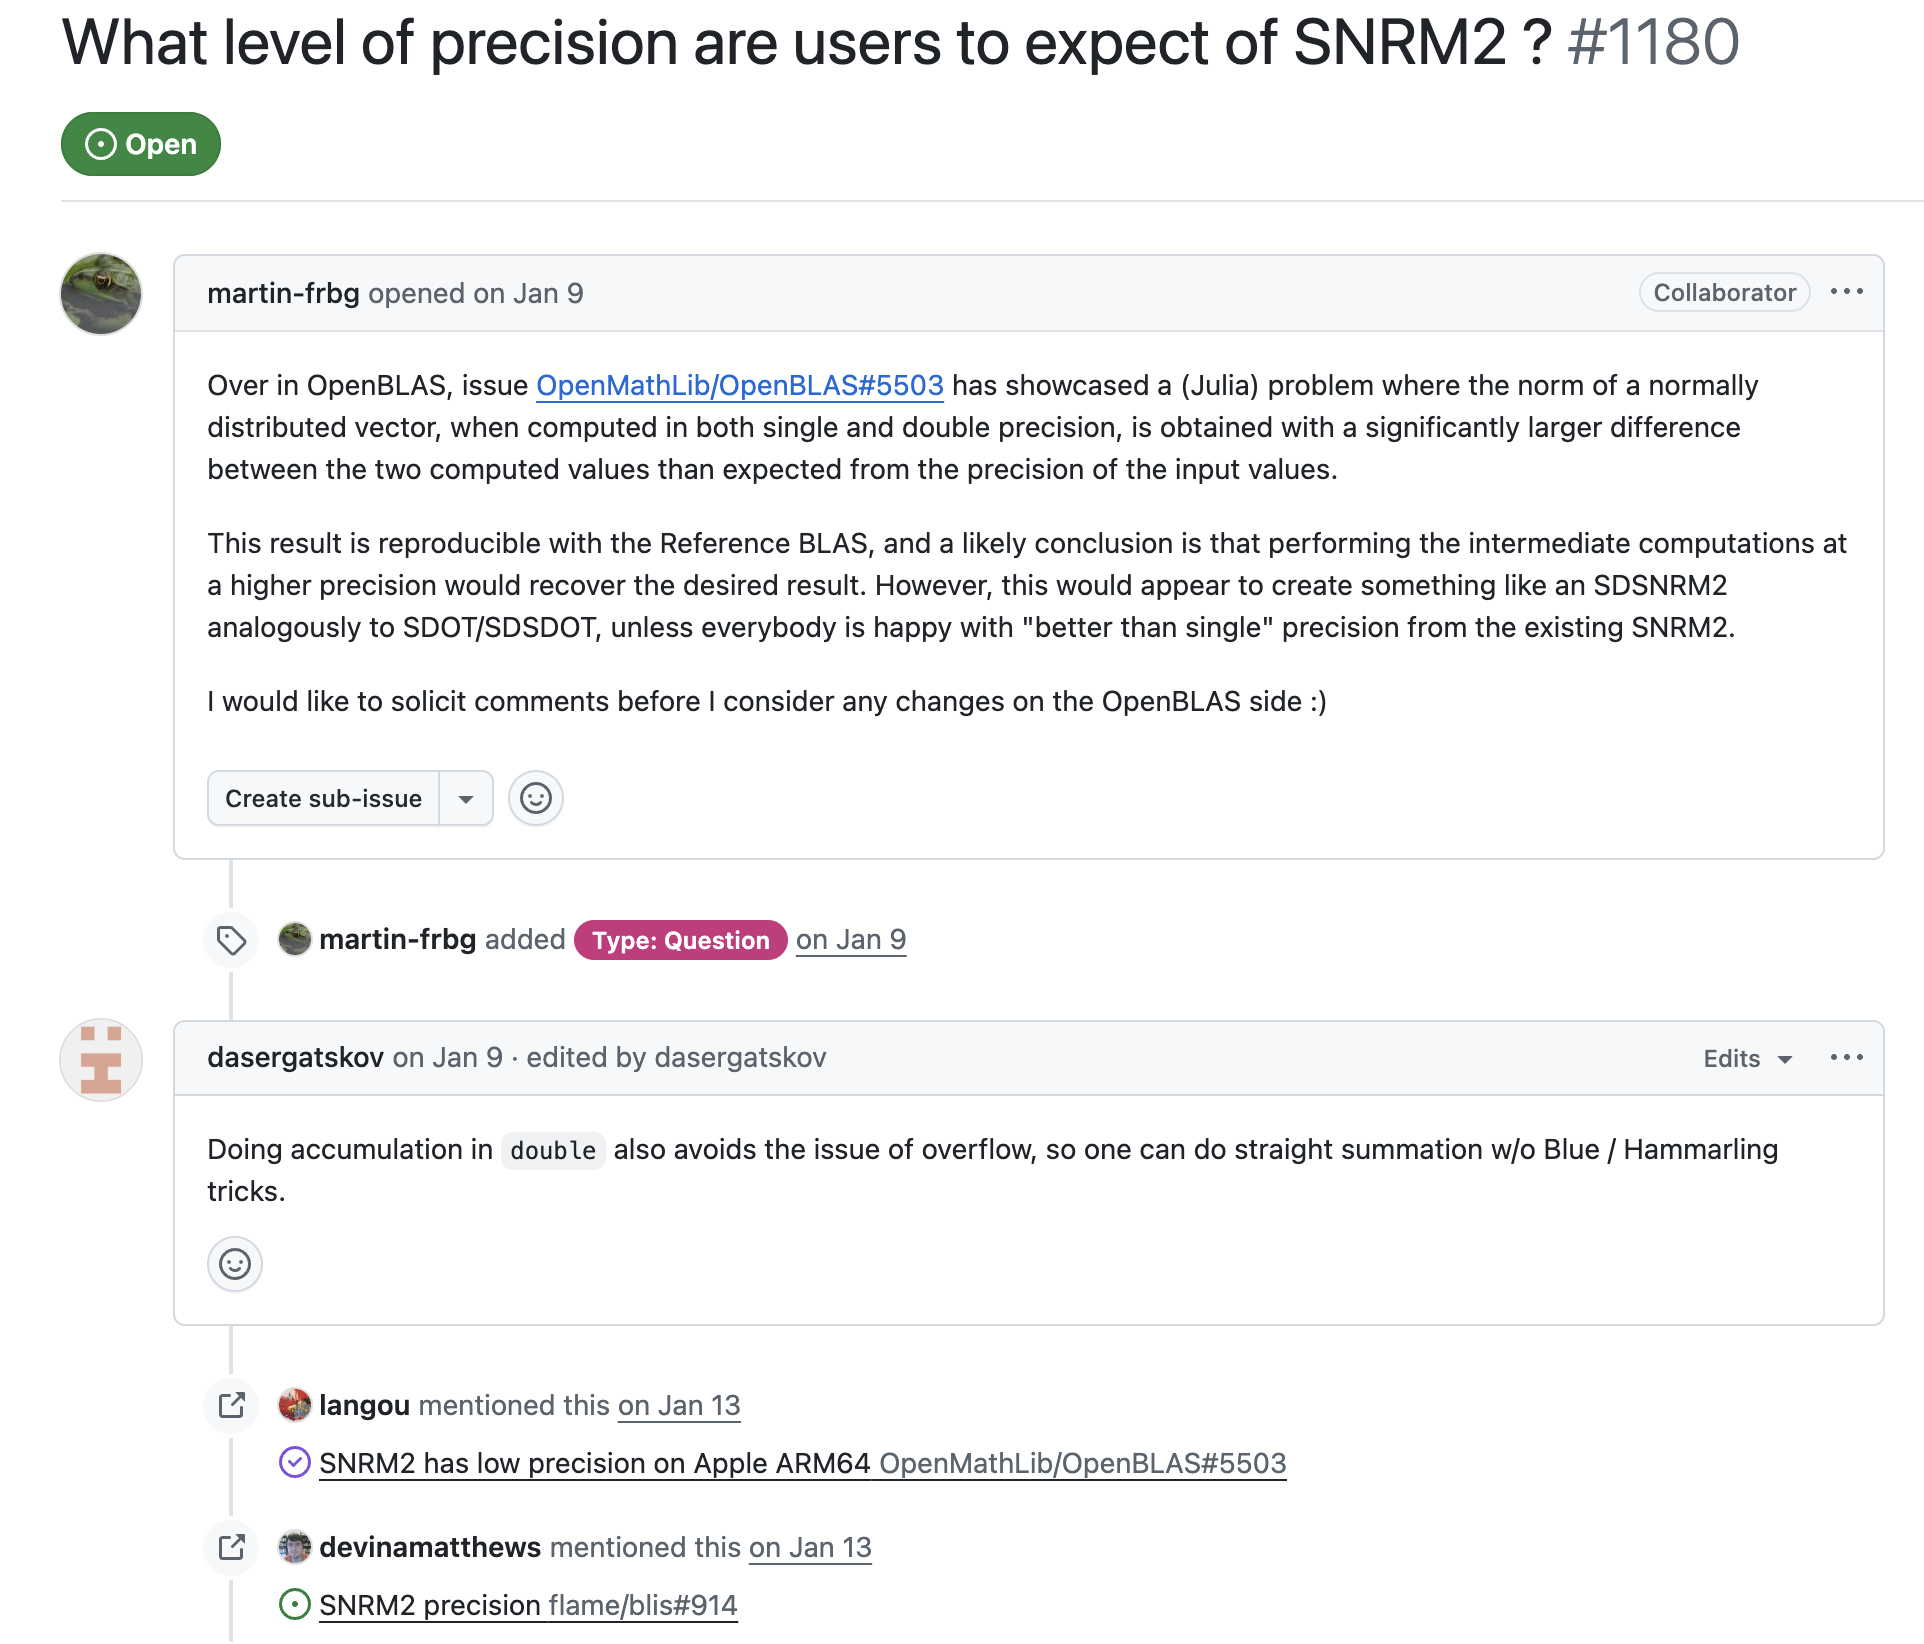
\includegraphics[width=\textwidth]{screenshots/SNRM2.png}

\end{frame}


\begin{frame}{accumulation in BLAS (2/3)}

%\href{https://github.com/Reference-LAPACK/lapack/issues/1180}{1180}
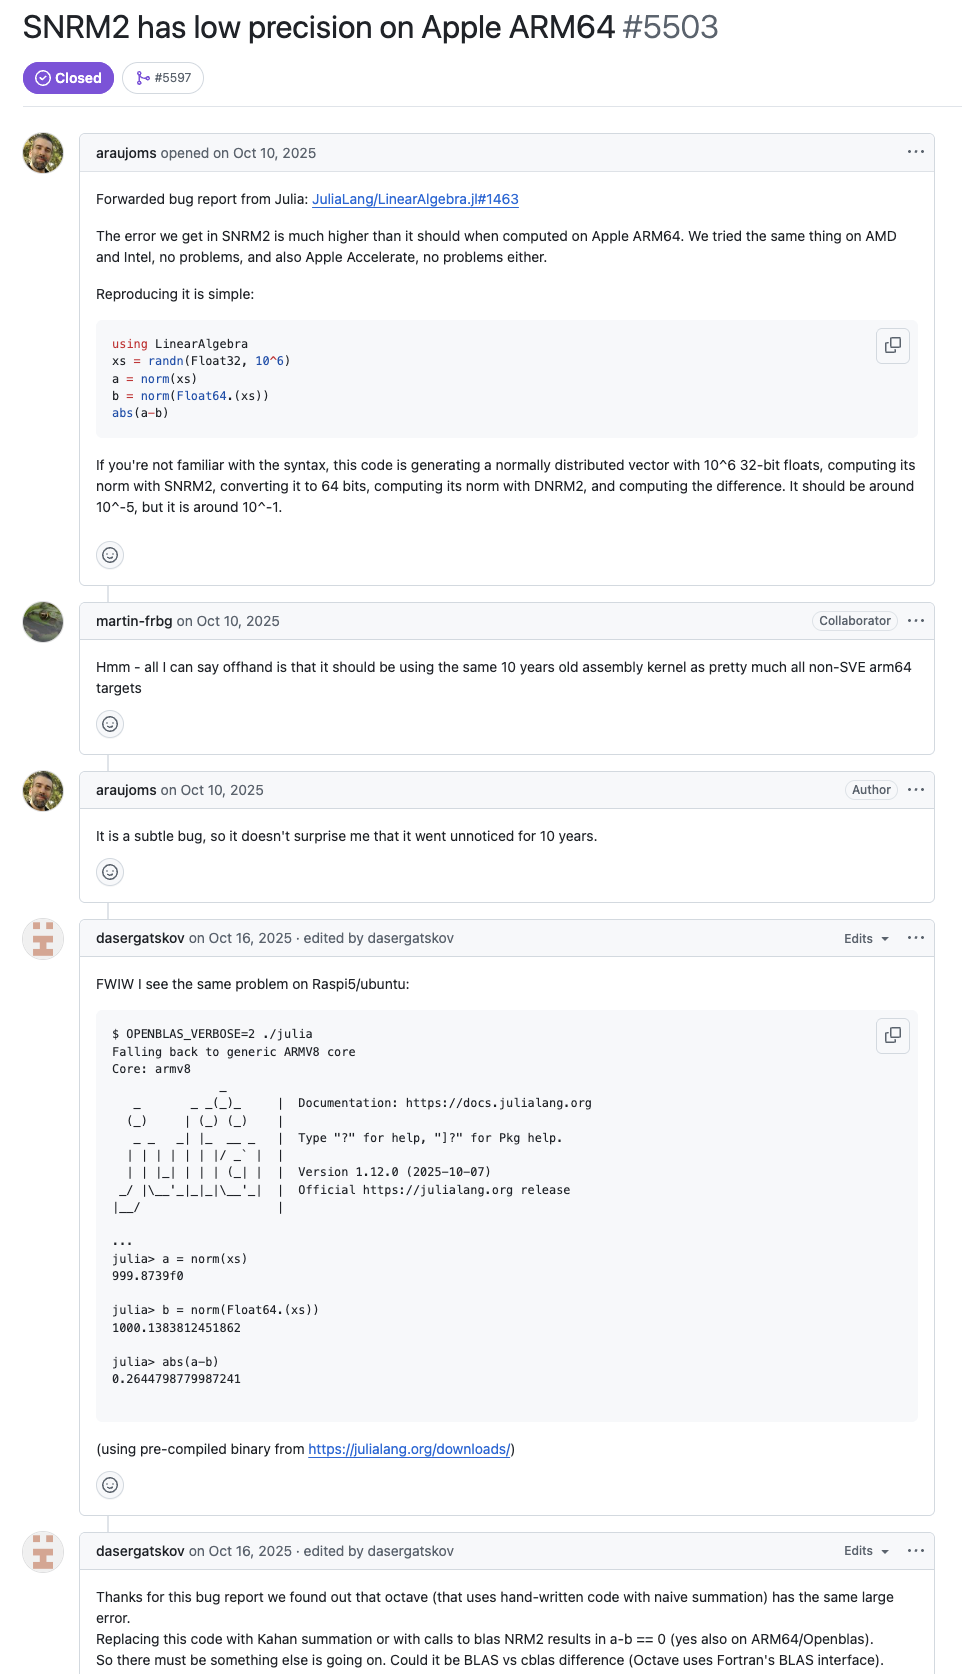
\includegraphics[height=.7\textheight]{screenshots/SNRM2-2.png}

\end{frame}


\begin{frame}{accumulation in BLAS (3/3)}

\pgfuseimage{beamericonarticle}~P. Blanchard, N. J. Higham, and T. Mary.
A Class of Fast and Accurate Summation Algorithms.
SIAM Journal on Scientific Computing 42(3):A1541-A1557, 2020.
DOI=\href{https://doi.org/10.1137/19M1257780}{10.1137/19M1257780}.


\end{frame}

\begin{frame}{DGMM}
%\href{https://github.com/Reference-LAPACK/lapack/issues/1178}{1178}
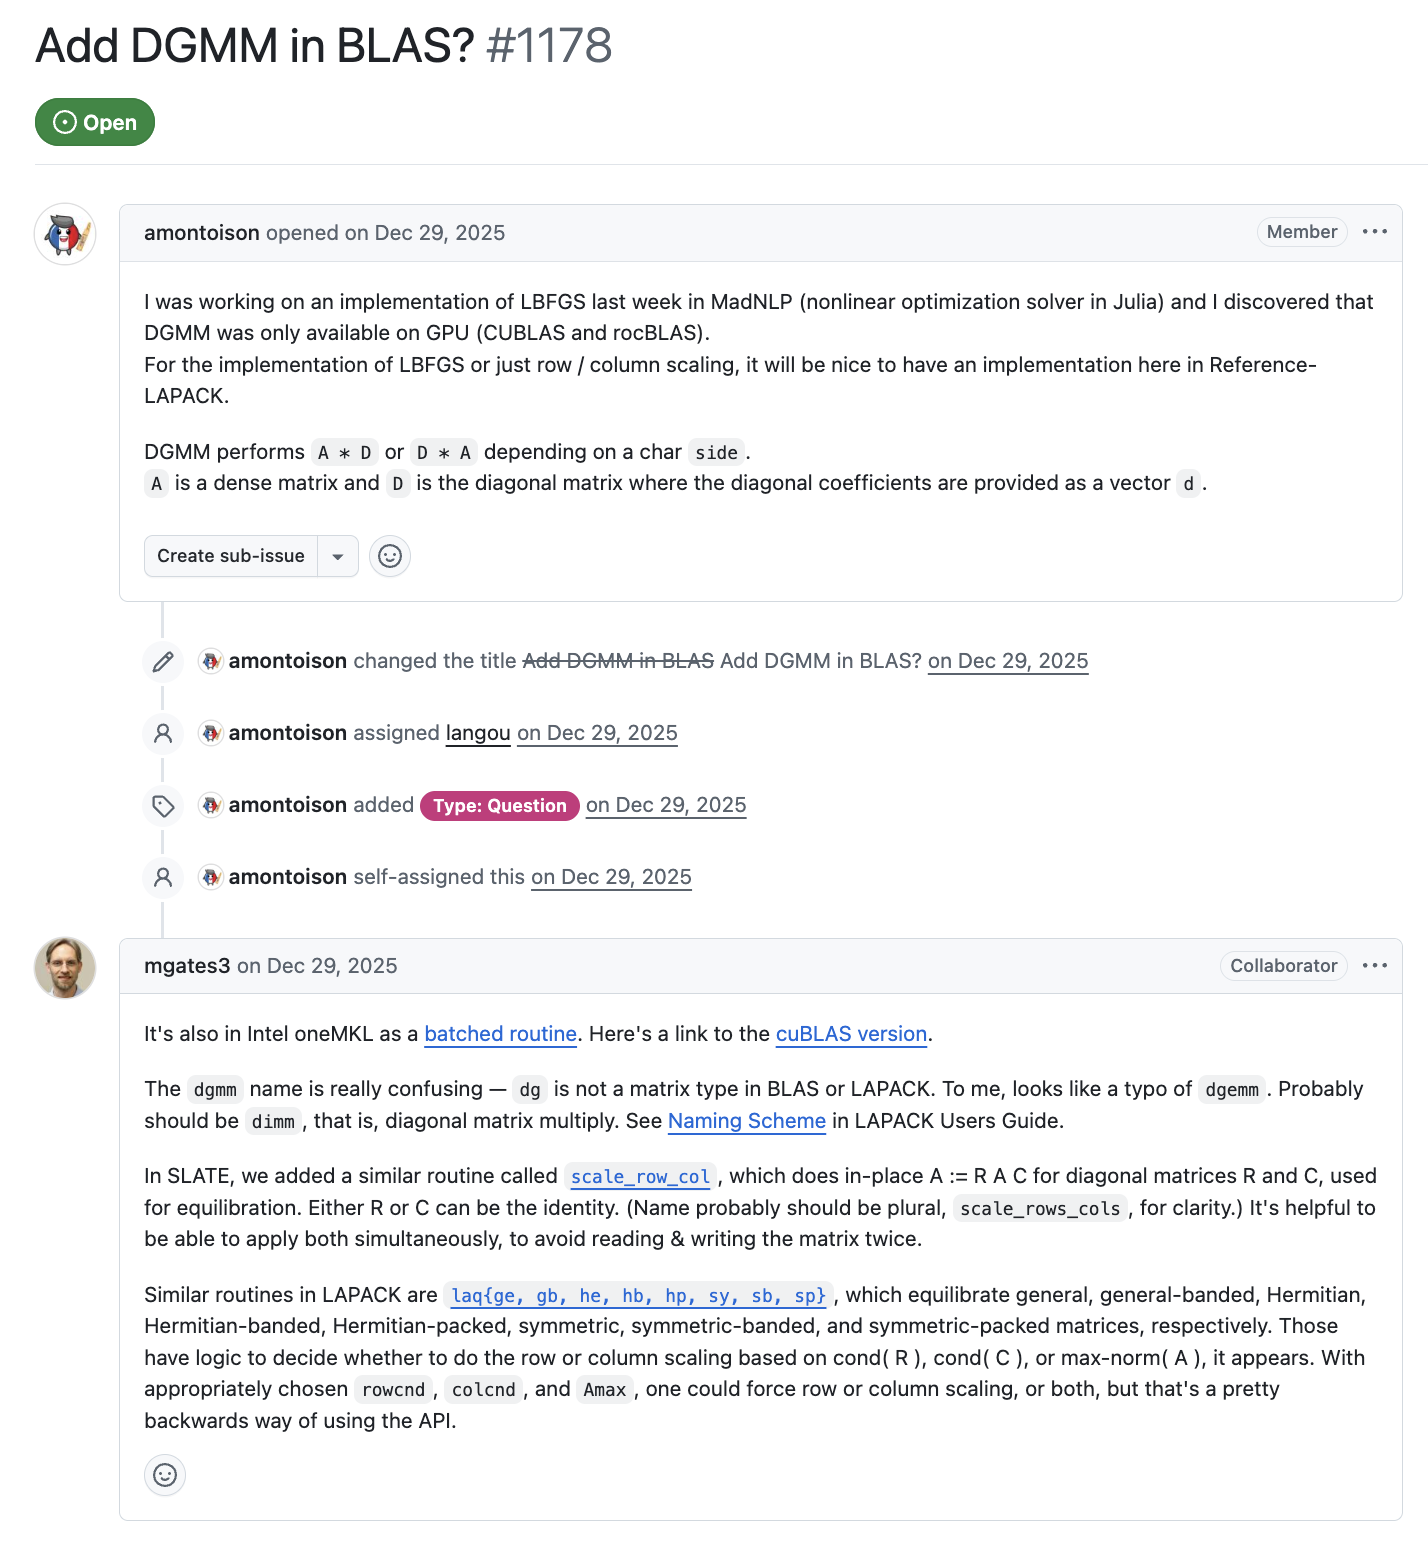
\includegraphics[height=\textheight]{screenshots/DGMM.png}
\end{frame}

\begin{frame}{CRSCL}
%Reciprocal Scaling of complex vectors. [C/Z]RSCL multiplies an n-element complex vector x by the complex scalar 1/a. This is done without overflow or underflow as long as the final result x/a does not overflow or underflow. See PR\#839
%\href{https://github.com/Reference-LAPACK/lapack/issues/839}{839}
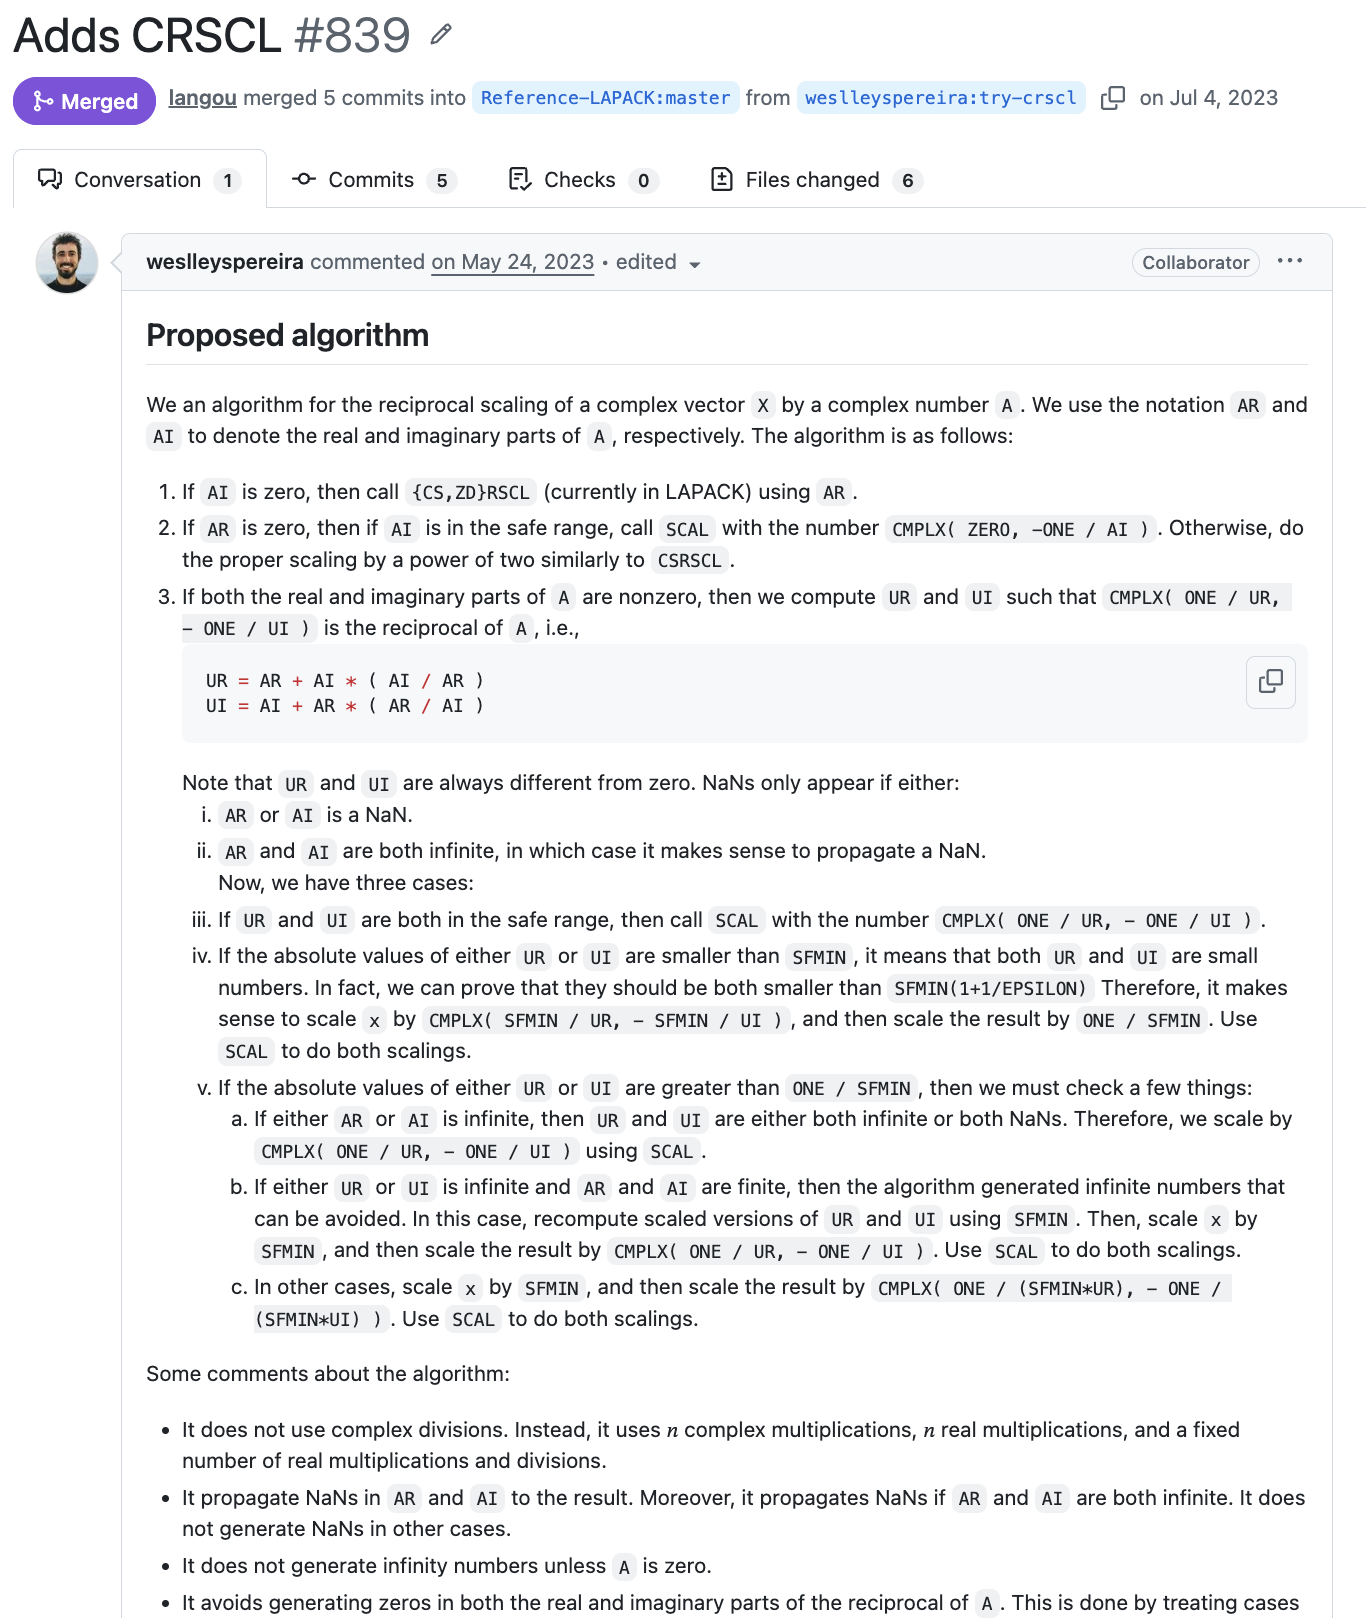
\includegraphics[height=\textheight]{screenshots/CRSCL.png}
\end{frame}



\begin{frame}{ROTC: chain of sequence of Givens rotations (1/3)}
%\href{https://github.com/Reference-LAPACK/lapack/pull/1067}{PR-1067}
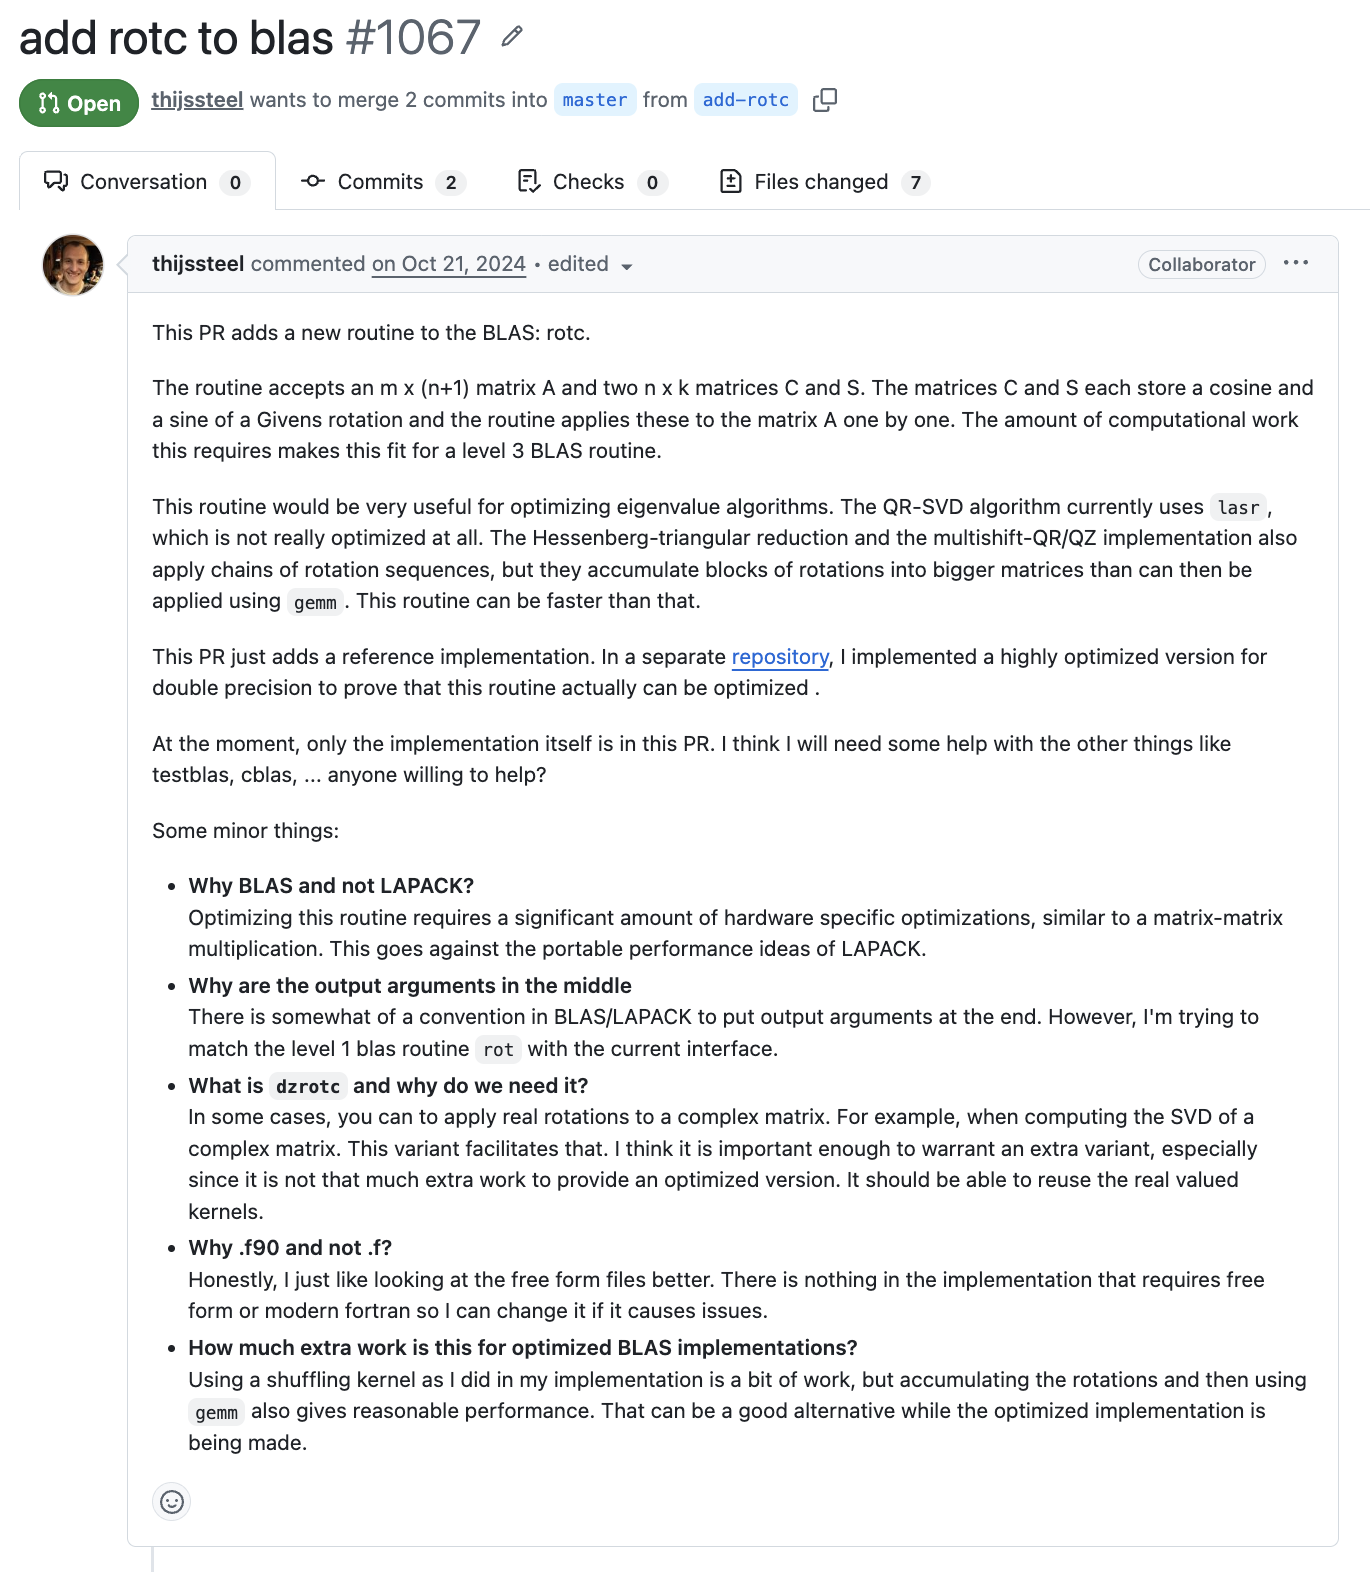
\includegraphics[height=\textheight]{screenshots/ROTC.png}

\end{frame}



\begin{frame}{ROTC: chain of sequence of Givens rotations (2/3)}
%\href{https://github.com/Reference-LAPACK/lapack/pull/1067}{PR-1067}
%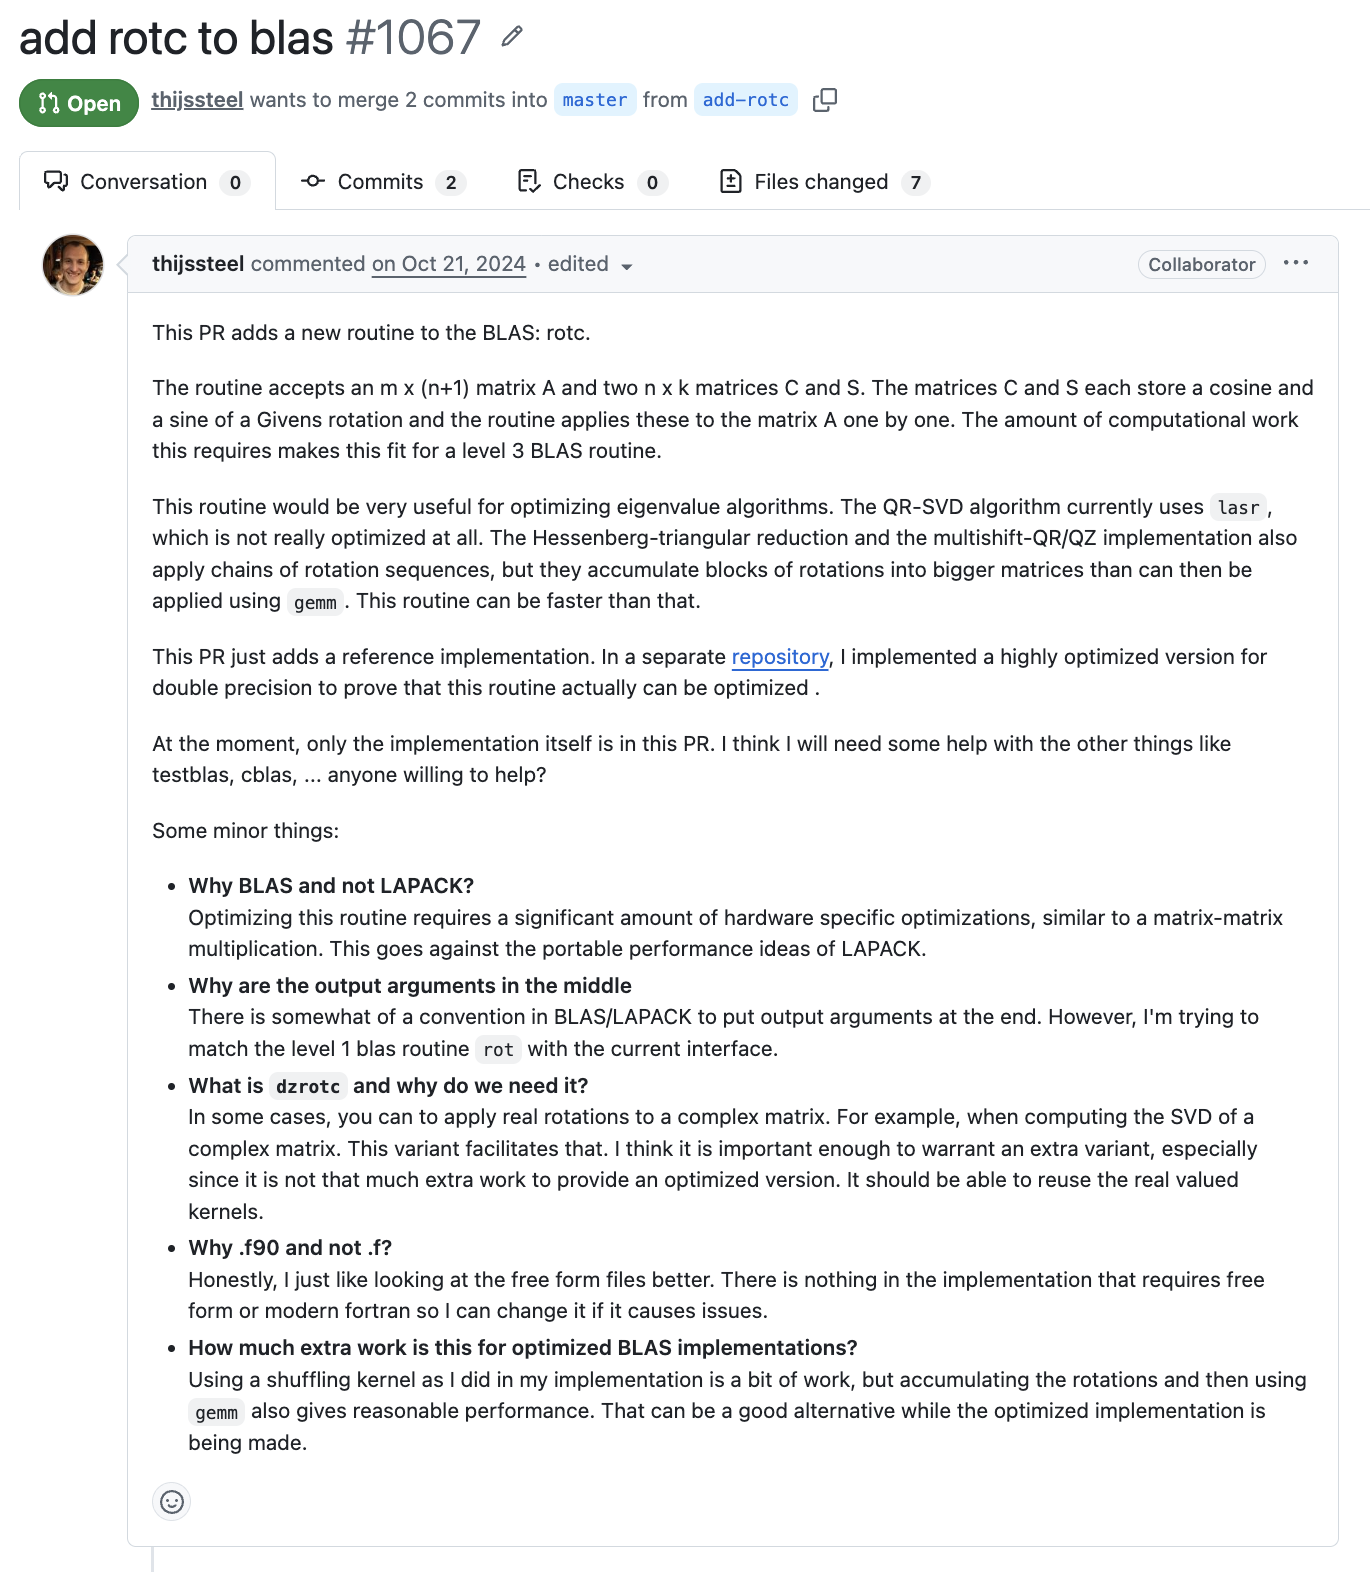
\includegraphics[height=\textheight]{screenshots/ROTC.png}

\pgfuseimage{beamericonarticle}~T. Steel and J. Langou.
Communication efficient application of sequences of planar rotations to a matrix.
arXiv:2412.01852, 2024.
% url={https://arxiv.org/abs/2412.01852}, 

\pgfuseimage{beamericonarticle}~F. G. Van Zee, R. A. van de Geijn, and G. Quintana-Ort{\'\i}. 
Restructuring the tridiagonal and bidiagonal QR algorithms for performance. 
ACM Transactions on Mathematical Software (TOMS), 40 (2014), pp. 1–34.


\end{frame}


\begin{frame}{ROTC: chain of sequence of Givens rotations (3/3)}
%\href{https://github.com/Reference-LAPACK/lapack/pull/1067}{PR-1067}
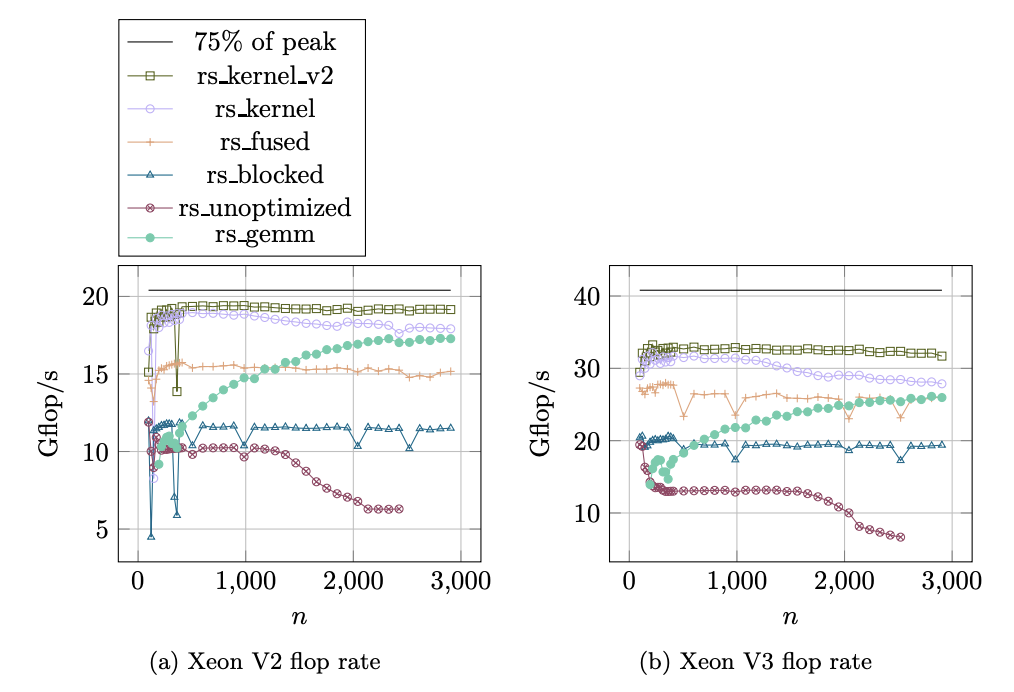
\includegraphics[height=\textheight]{screenshots/ROTC-2.png}

\end{frame}




\begin{frame}{Batch BLAS}
%\href{https://github.com/Reference-LAPACK/lapack/pull/916}{PR-916}
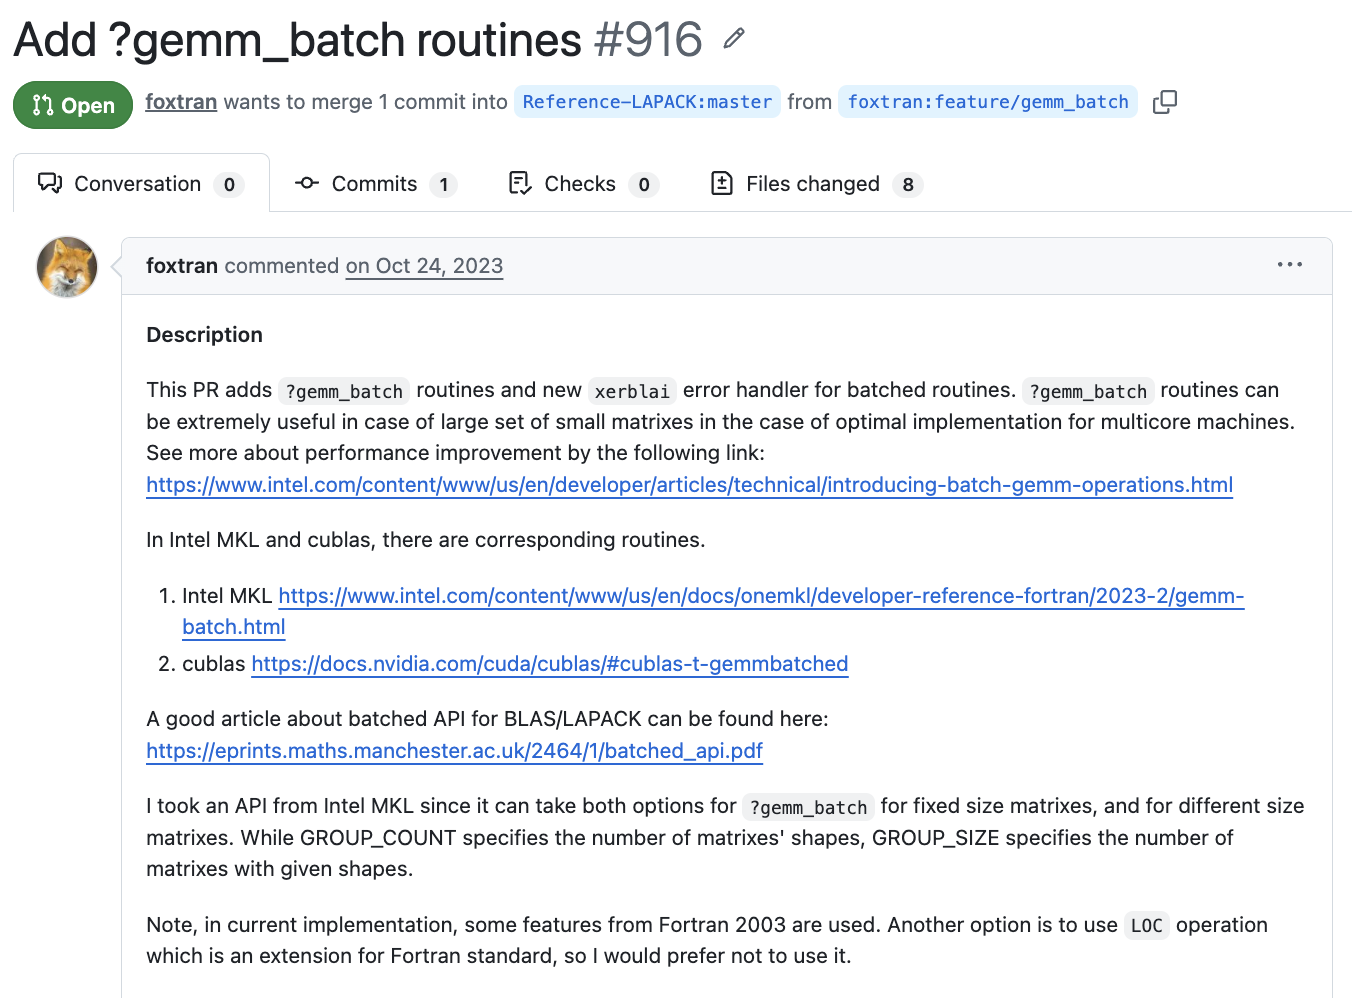
\includegraphics[height=\textheight]{screenshots/batched.png}
\end{frame}


\begin{frame}{inplace transposition}
%\href{https://github.com/Reference-LAPACK/lapack/issues/1017}{ISSUE-1017}
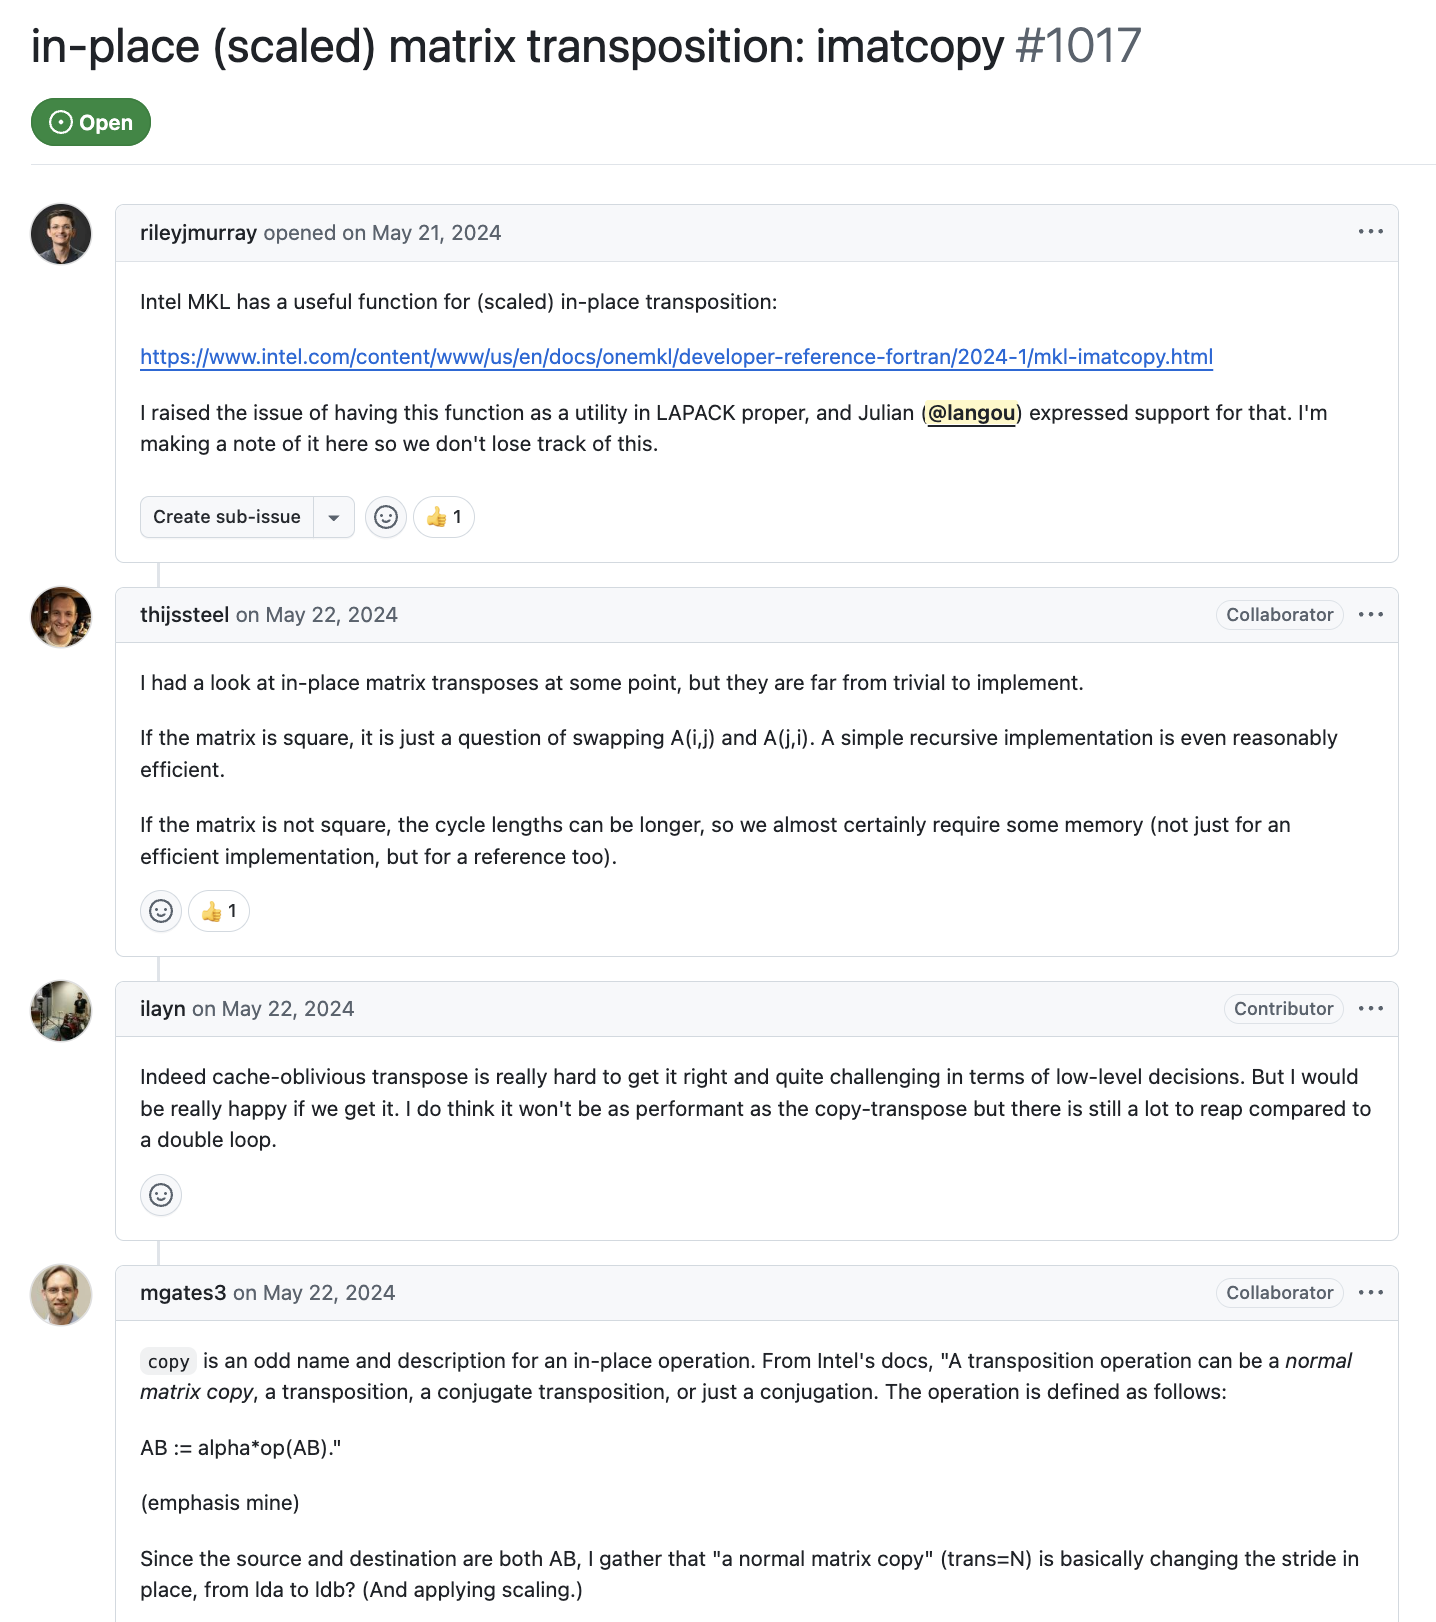
\includegraphics[height=\textheight]{screenshots/inplace-transpose.png}
\end{frame}

\begin{frame}{sandwich operators}
%\href{https://github.com/Reference-LAPACK/lapack/issues/1017}{ISSUE-1017}

$$ C \leftarrow \alpha A X A^H + \beta C $$

with $X$ diagonal real, 
Hermitian diagonal with 1x1 or 2x2 blocks,
Hermitian tridiagonal. 

\end{frame}

\begin{frame}{even more flags (1/3)}
%\href{https://github.com/Reference-LAPACK/lapack/issues/1017}{ISSUE-1017}
Extract of zpotf2.f\\
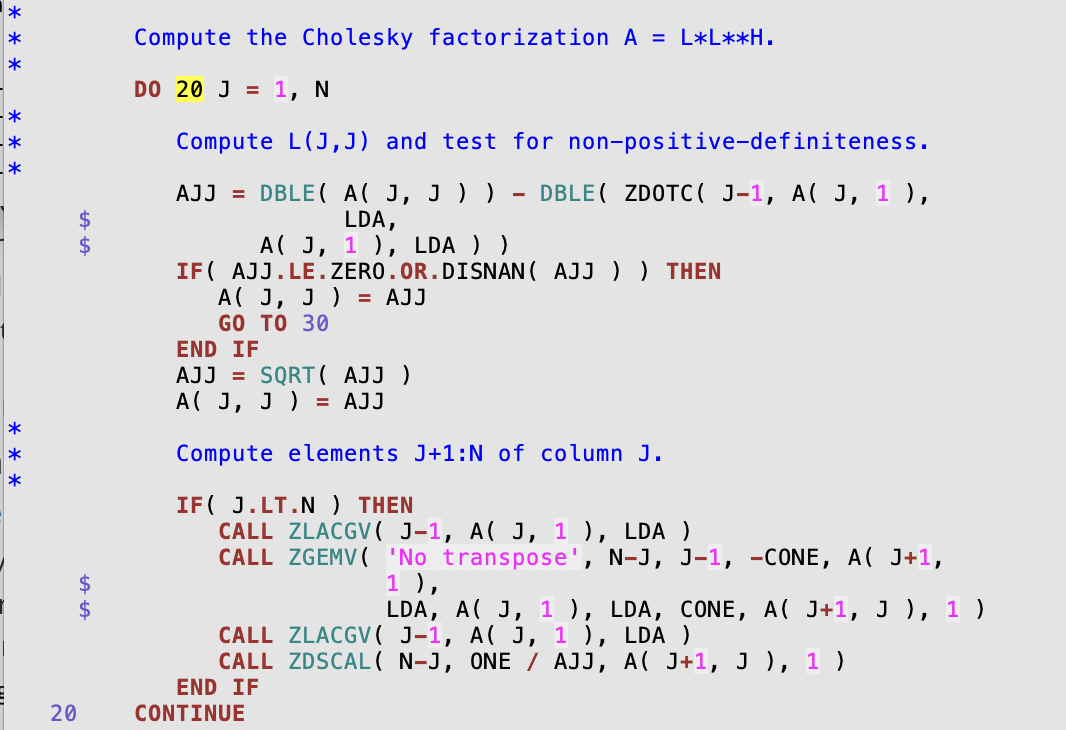
\includegraphics[height=.7\textheight]{screenshots/zpotf2.png}
\end{frame}

\begin{frame}{even more flags (2/3)}
% email from Johnathan

AXCPY

$$ y \leftarrow \alpha x^H + y$$

%\begin{verbatim}
%DO I = 1, LASTC
%Y(I) = Y(I) + ALPHA * DCONJG(X(I))
%END DO
%\end{verbatim}

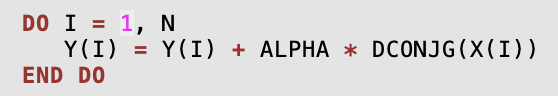
\includegraphics[width=.7\textwidth]{screenshots/loop.png}


\end{frame}

\begin{frame}{even more flags (3/3)}
%\href{https://github.com/Reference-LAPACK/lapack/issues/1017}{ISSUE-1017}
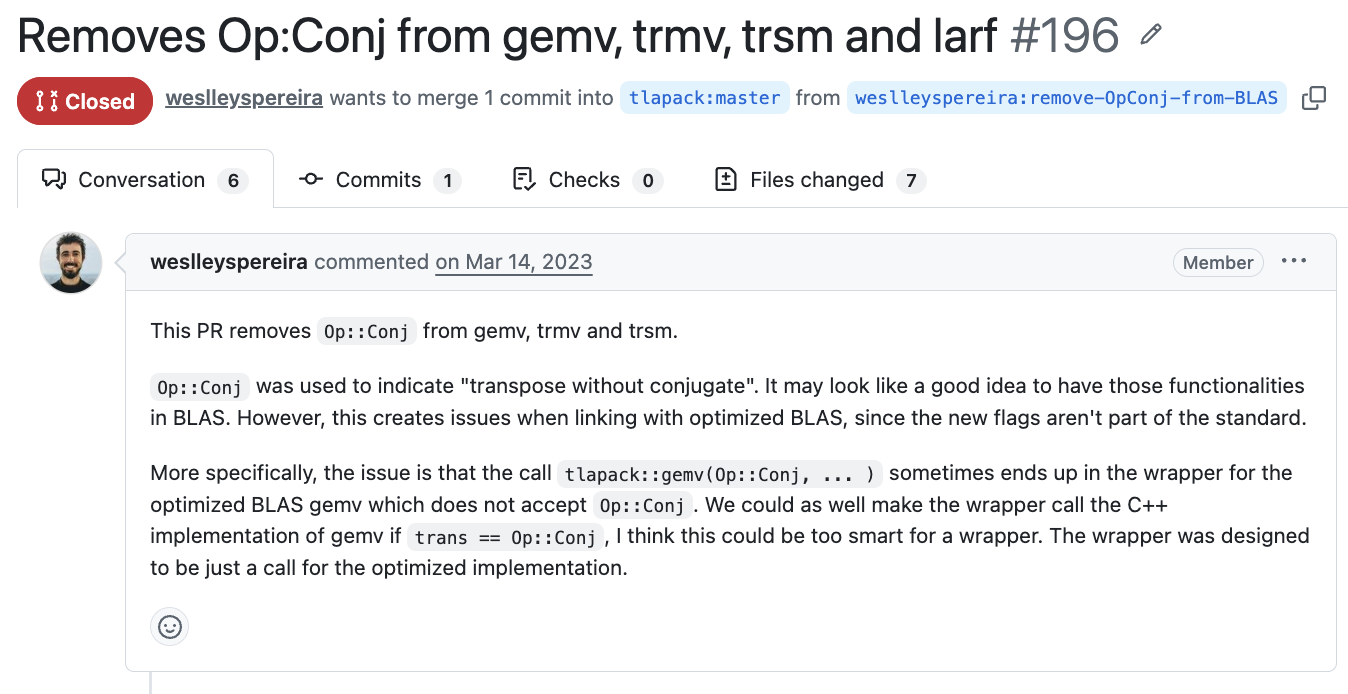
\includegraphics[height=\textheight]{screenshots/moreflags.png}
\end{frame}

%\begin{frame}{even more flags (3/3)}

% FROM RHYNE

% > The main issue that arose was assuming v(1)=1 means in the HC case of
% > zlarf we have to compute the following
% >
% > (I-tvv**H)C = C -tvv**HC
% >
% > First we compute w**H = v**HC or w = C**Hv = C_1**H + C_2**Hv_2
% >
% > I think we need to do that conjugate transpose as zgemv does not have
% > an option to do a left multiply by a vector (possibly different
% > routine) and doesn't allow us to conjugate the vector only the matrix

% \end{frame}


\begin{frame}{TRTRM}
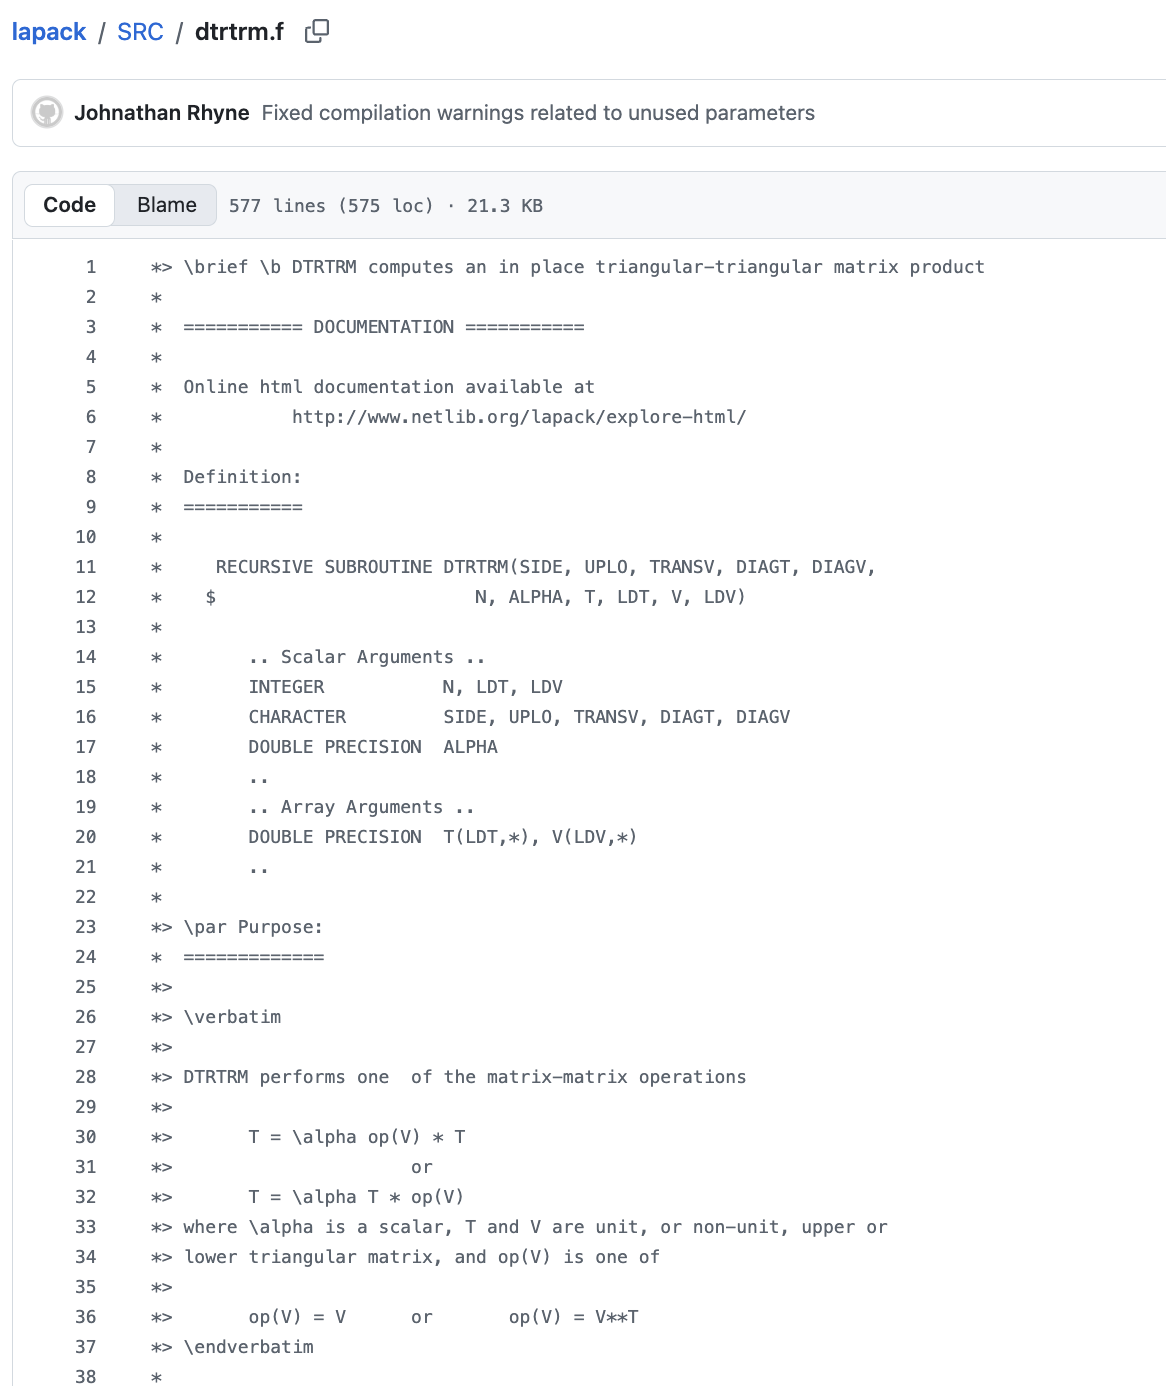
\includegraphics[height=.7\textheight]{screenshots/TRTRM.png}
\end{frame}


\begin{frame}{LLH and UUH and LAUUM}
\begin{tabular}{cc}
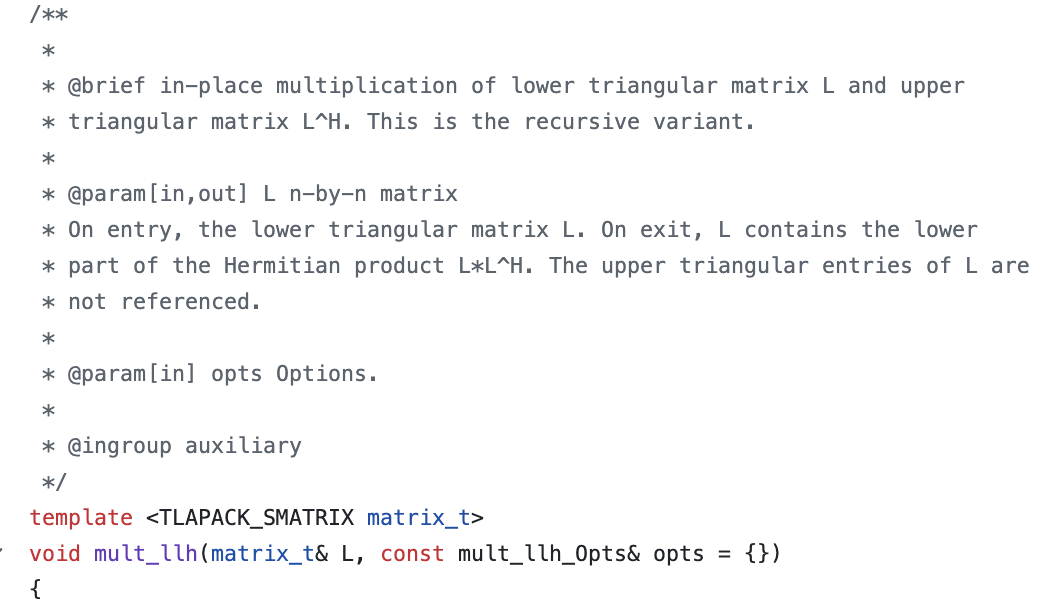
\includegraphics[width=.5\textwidth]{screenshots/llh.png}&
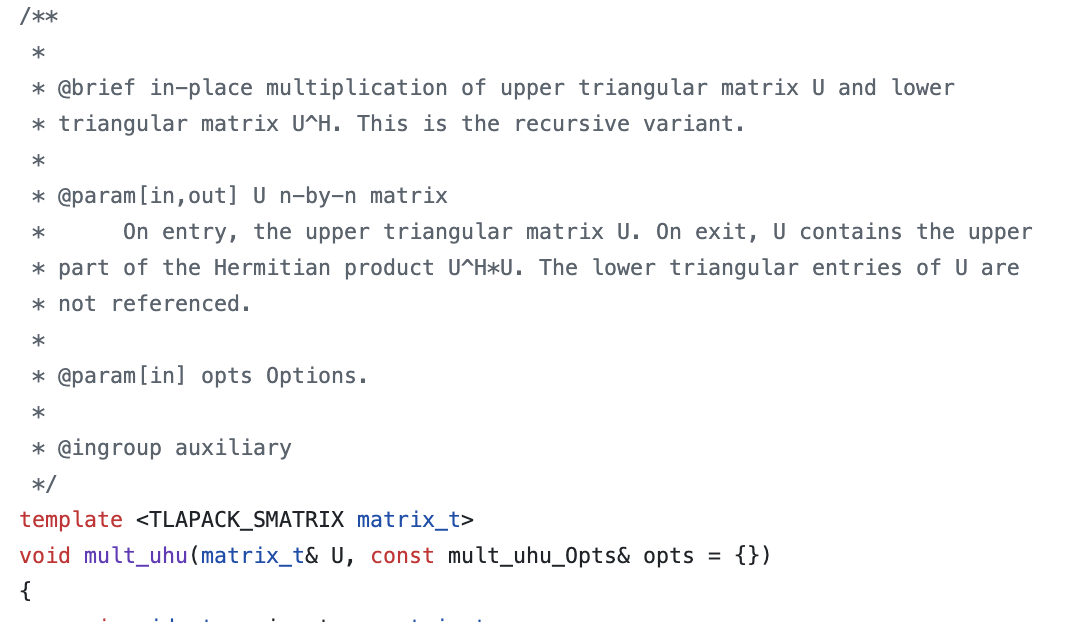
\includegraphics[width=.5\textwidth]{screenshots/uhu.png}
\end{tabular}
%https://github.com/tlapack/tlapack/blob/master/include/tlapack/lapack/mult_llh.hpp
%https://github.com/tlapack/tlapack/blob/master/include/tlapack/lapack/mult_uhu.hpp
%https://github.com/tlapack/tlapack/blob/master/include/tlapack/lapack/lauum_recursive.hpp
\end{frame}


\begin{frame}{TRTRM\_OUT}
%\href{https://github.com/tlapack/tlapack/blob/master/include/tlapack/lapack/trmm_out.hpp}{include/tlapack/lapack/trmm\_out.hpp}
\begin{tabular}{cc}
\begin{minipage}{.2\textwidth}
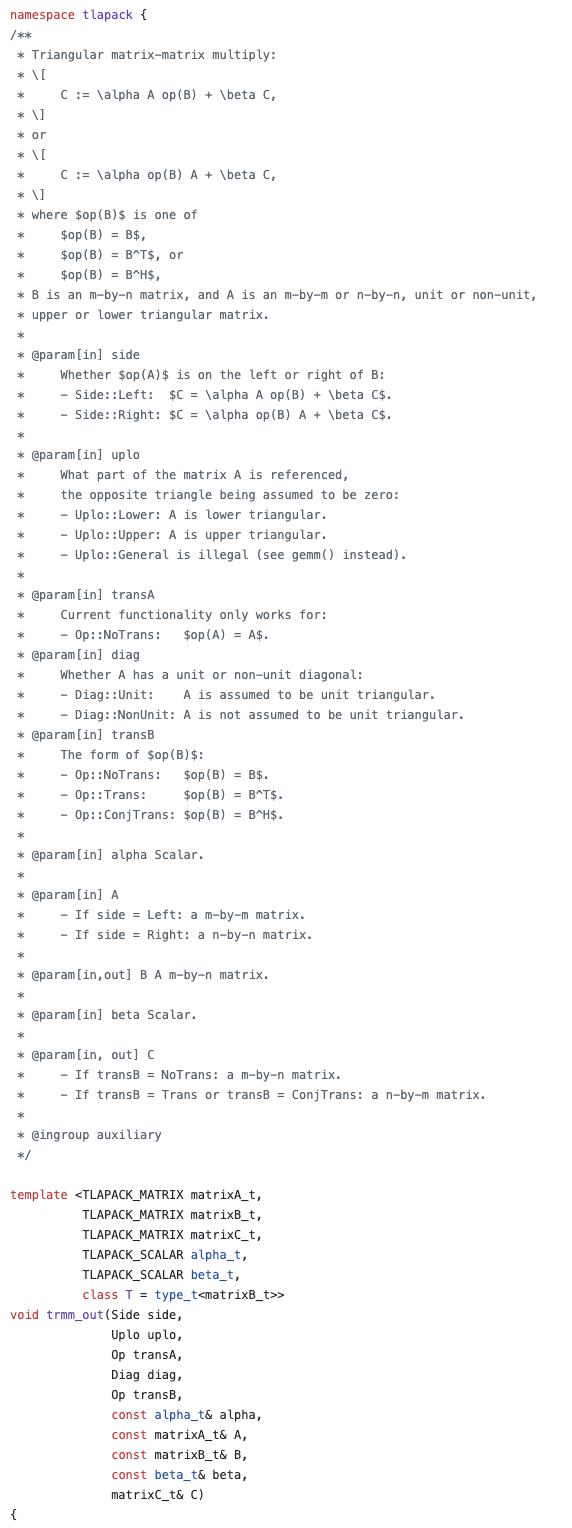
\includegraphics[width=\textwidth]{screenshots/TRMM_OUT.png}
\end{minipage}&
\begin{minipage}{.5\textwidth}
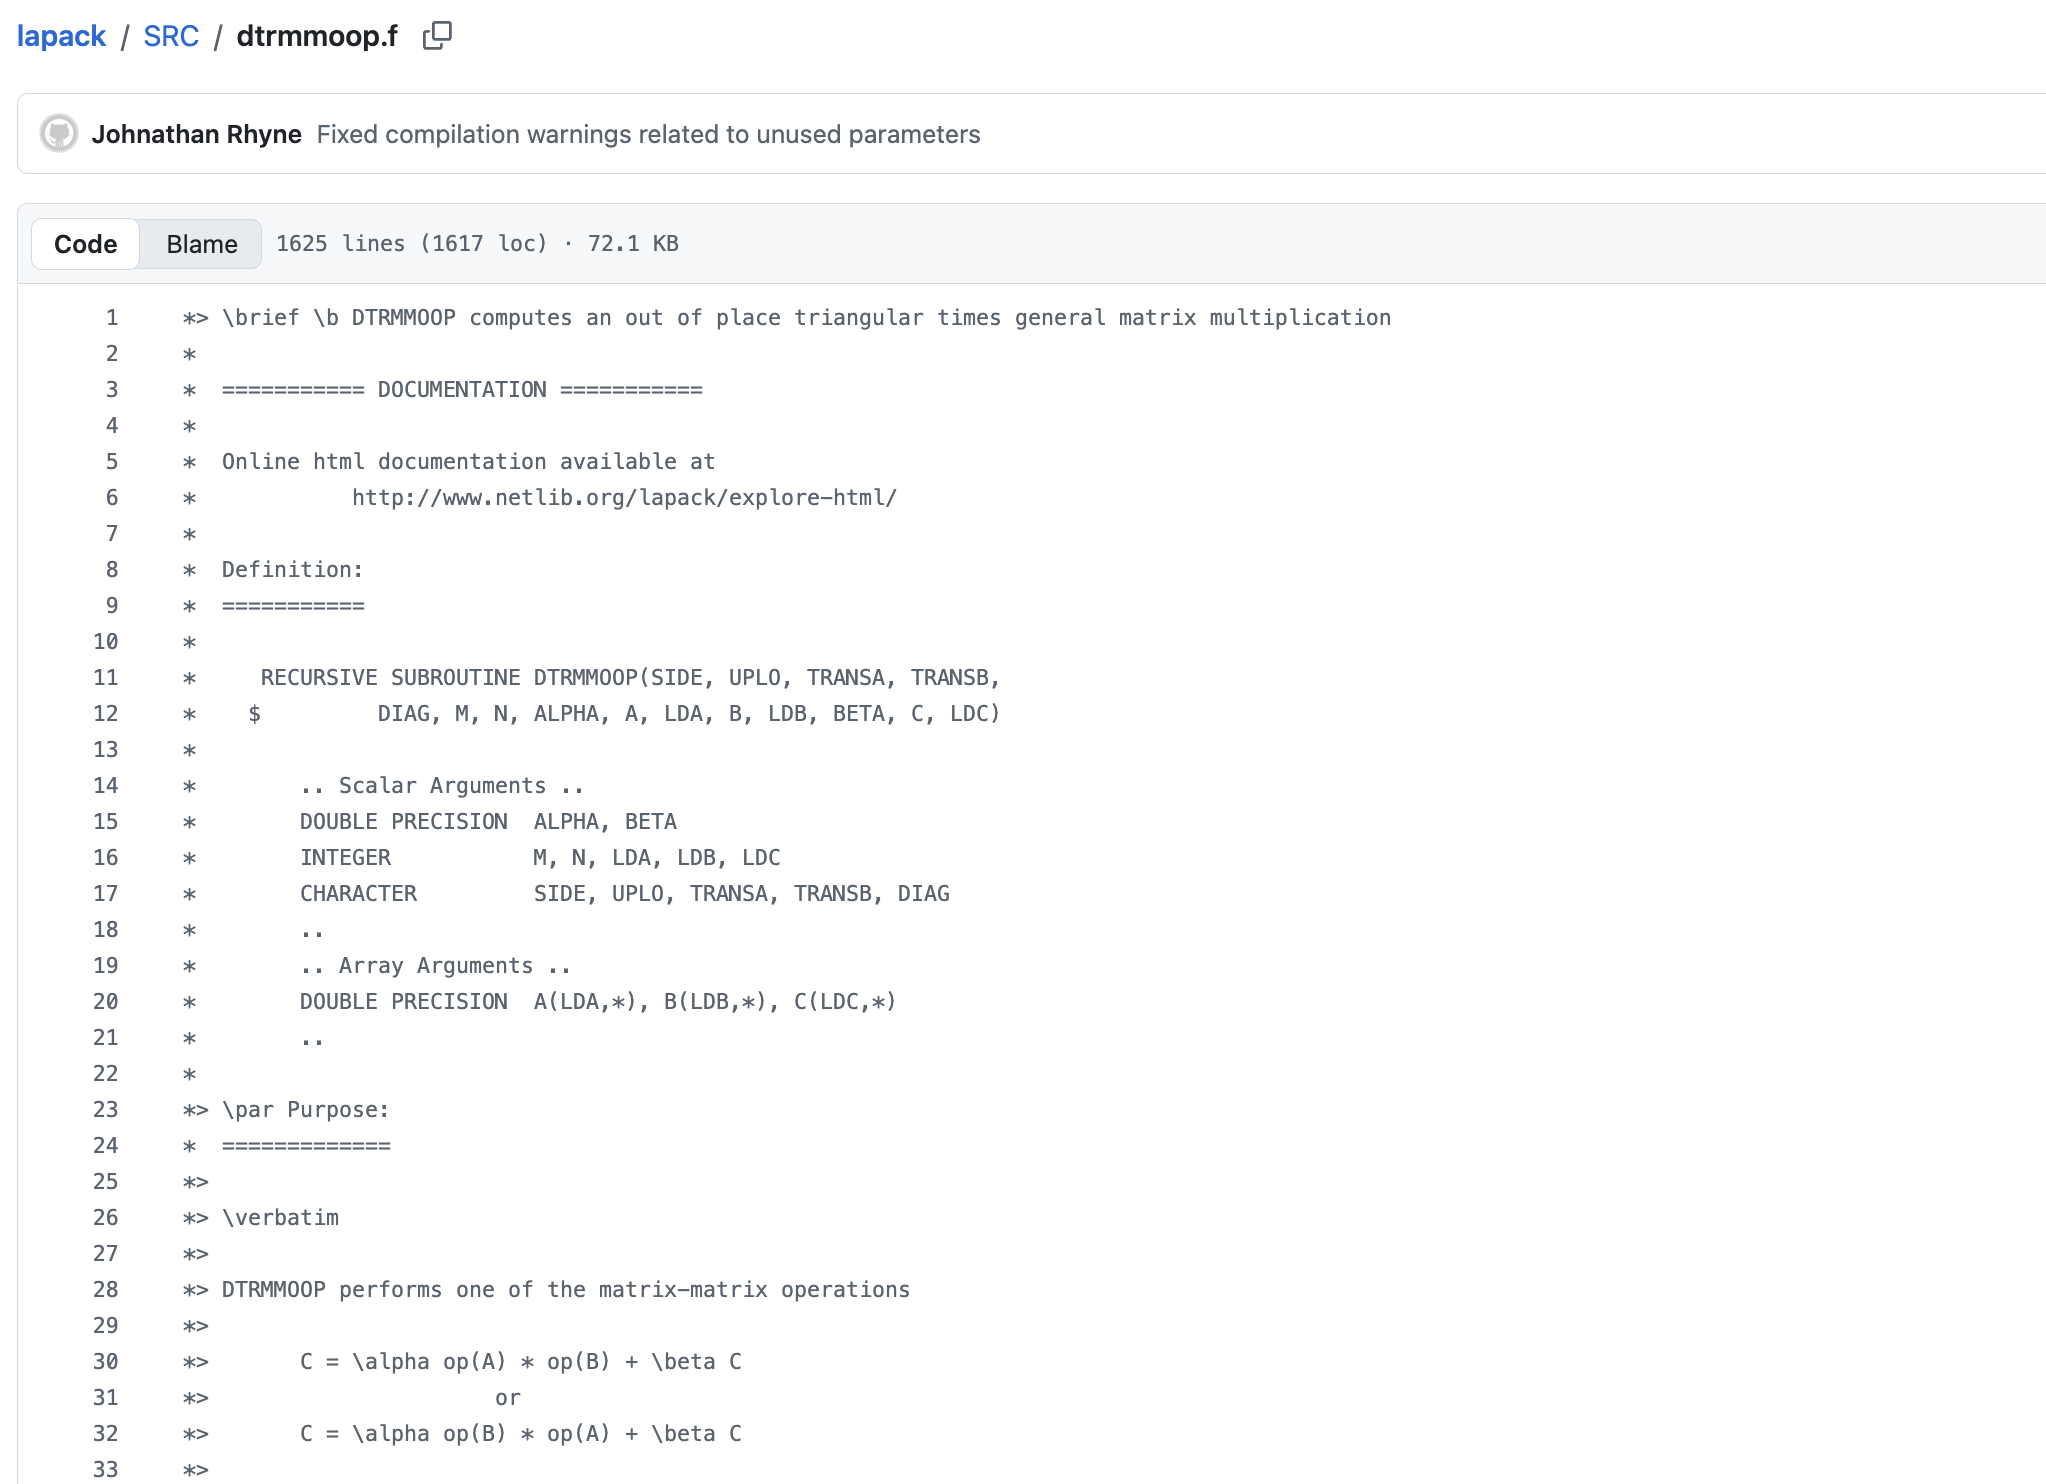
\includegraphics[width=\textwidth]{screenshots/TRMMOOP.png}
\end{minipage}
\end{tabular}
\end{frame}

\begin{frame}{LUMM}
%\href{https://github.com/jprhyne/lapack/blob/master/SRC/dlumm.f}{https://github.com/jprhyne/lapack/blob/master/SRC/dlumm.f}
\begin{tabular}{cc}
\begin{minipage}{.2\textwidth}
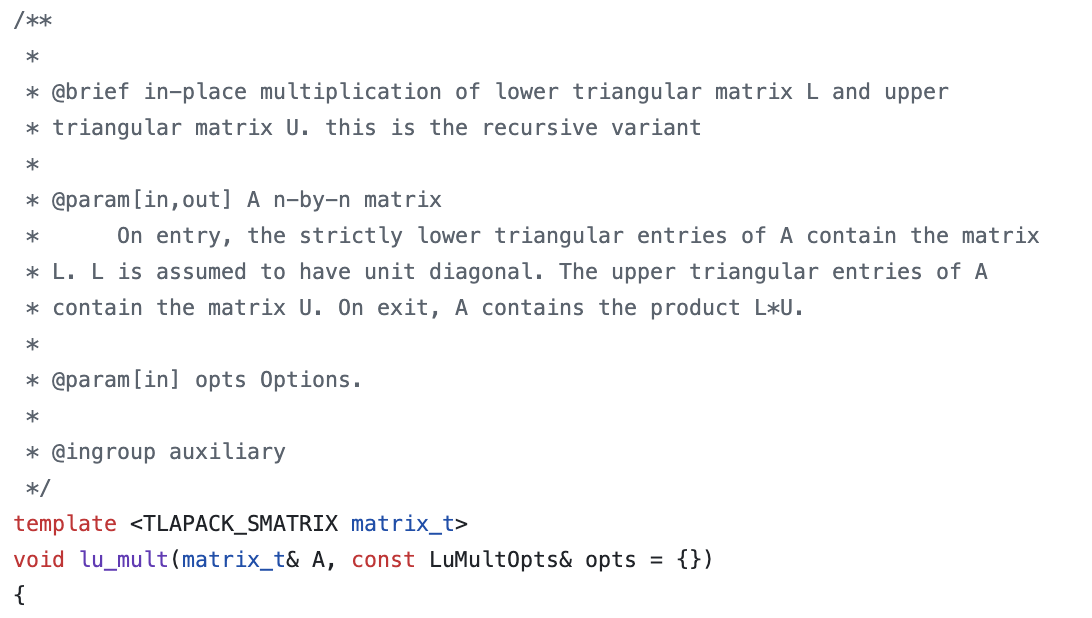
\includegraphics[width=\textwidth]{screenshots/lu_mult.png}
\end{minipage}&
\begin{minipage}{.5\textwidth}
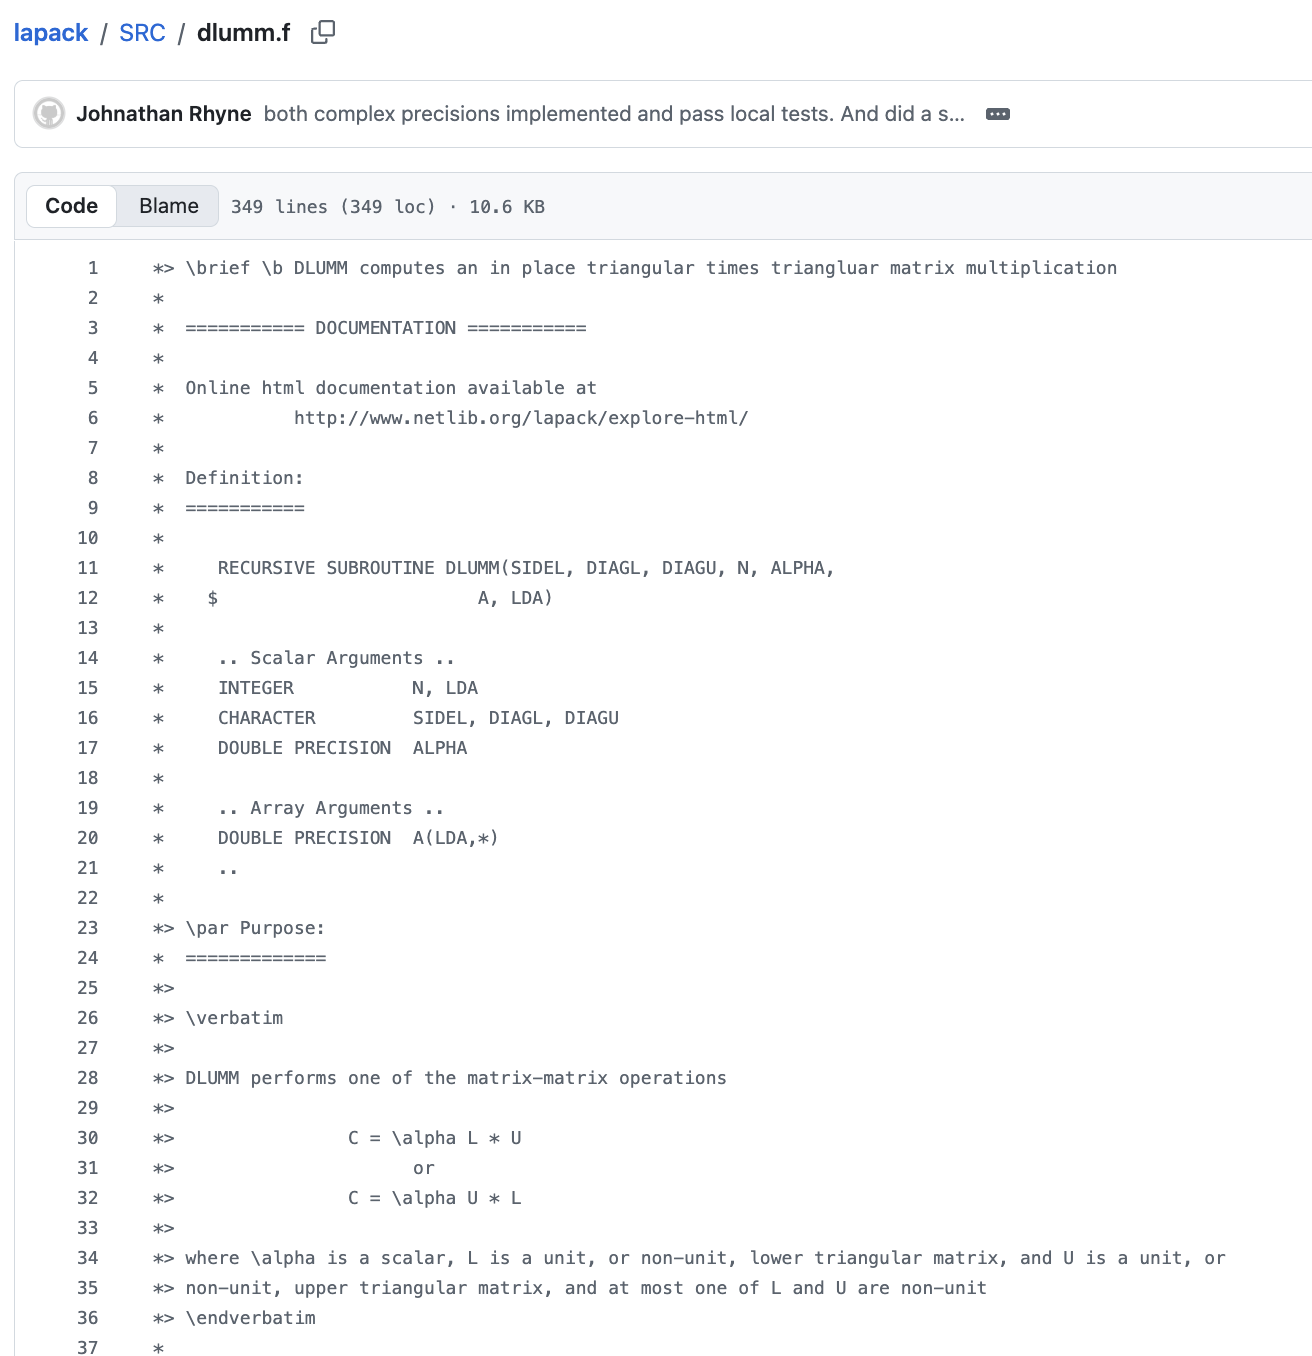
\includegraphics[height=.7\textheight]{screenshots/LUMM.png}
\end{minipage}
\end{tabular}
\end{frame}


\begin{frame}{ul\_mult}
%\href{https://github.com/jprhyne/lapack/blob/master/SRC/dlumm.f}{https://github.com/jprhyne/lapack/blob/master/SRC/dlumm.f}
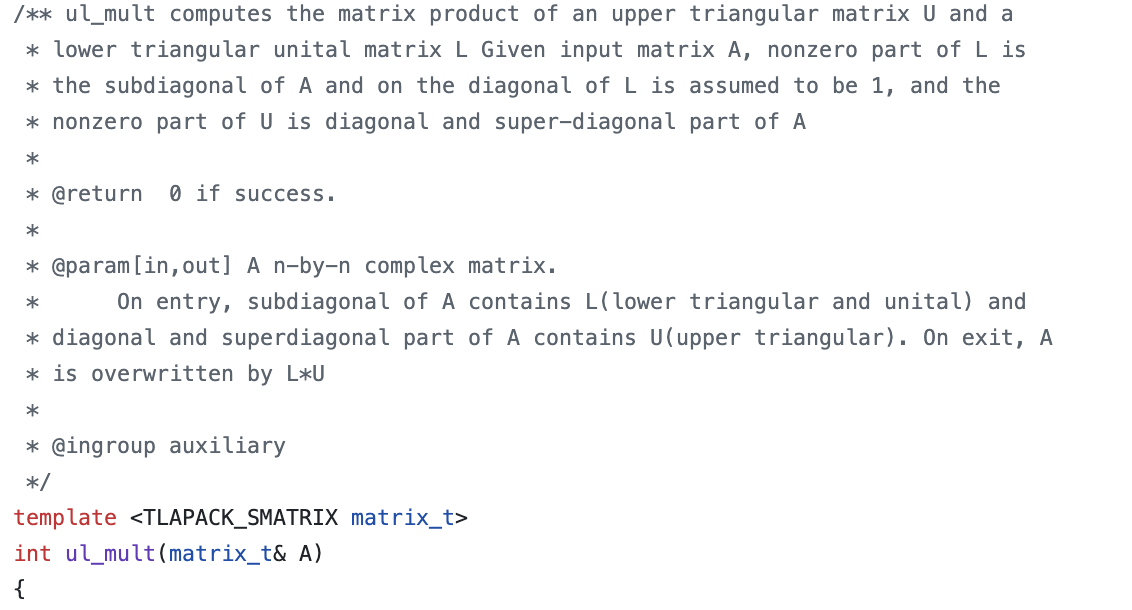
\includegraphics[height=.7\textheight]{screenshots/ul_mult.png}
\end{frame}




\begin{frame}{MULT\_HEHE}
%\href{https://github.com/Reference-LAPACK/lapack/issues/1017}{ISSUE-1017}
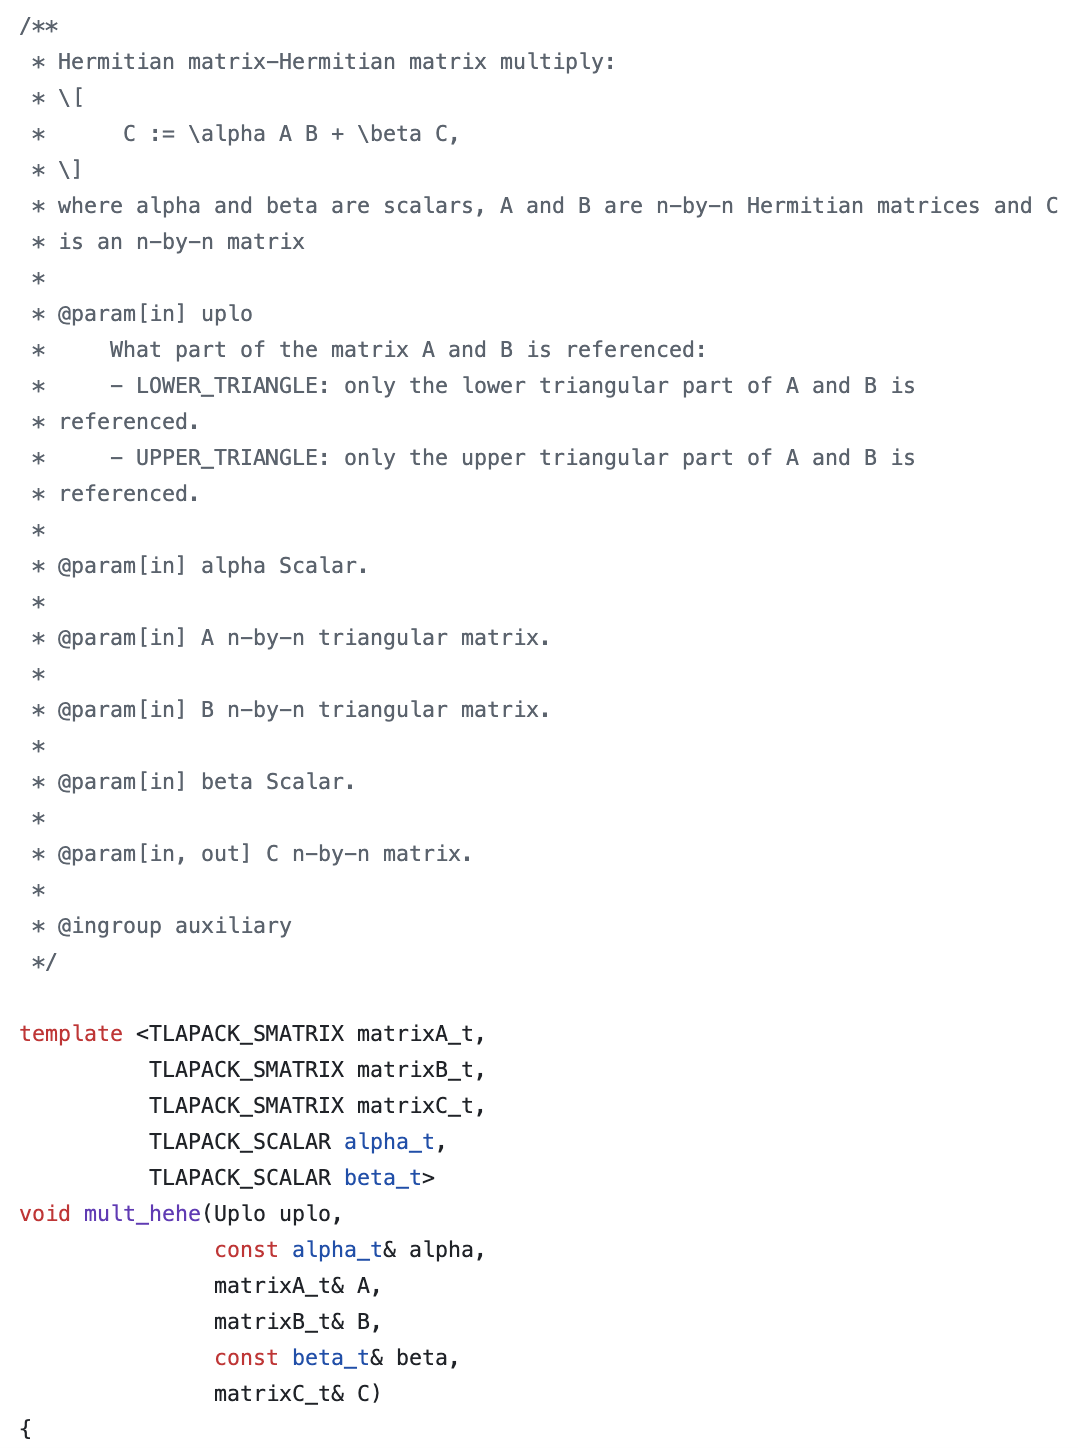
\includegraphics[height=.7\textheight]{screenshots/mult_hehe.png}
\end{frame}





% \begin{frame}{even more flags (3/3)}
% I feel we need some more triangular MM that are not in the BLAS.
% Lindsay and Naomi, both needed ( L = unit lower, in inout A ) * ( U = upper, in inout A ) ==> ( A = general, in inout A )
% Lindsay needed alpha * ( U = upper, in input U ) * ( A = general, in input A ) + beta ( C = general, in inout C ) ==> ( C = general, in inout C )
% Then Heidi needed
% ( A = lower, in input A ) * ( B = lower, in inout B ) ==> ( B = lower, in inout B )
% And
% ( L = lower, in input A ) * ( L^H = upper, in inout A ) ==> ( A = symmetric, lower part stored, in inout A )
% ( L^H = upper, in input A ) * ( L = lower, in inout A ) ==> ( A = symmetric, lower part stored, in inout A )
% ( U^H = lower, in input A ) * ( U = upper, in inout A ) ==> ( A = symmetric, upper part stored, in inout A )
% ( U = upper, in input A ) * ( U^H = lower, in inout A ) ==> ( A = symmetric, upper part stored, in inout A )
% So all these routines are being written now.
% \end{frame}


% \begin{frame}{even more flags (3/3)}
% I feel we need some more triangular MM that are not in the BLAS.
% Lindsay and Naomi, both needed ( L = unit lower, in inout A ) * ( U = upper, in inout A ) ==> ( A = general, in inout A )
% Lindsay needed alpha * ( U = upper, in input U ) * ( A = general, in input A ) + beta ( C = general, in inout C ) ==> ( C = general, in inout C )
% Then Heidi needed
% ( A = lower, in input A ) * ( B = lower, in inout B ) ==> ( B = lower, in inout B )
% And
% ( L = lower, in input A ) * ( L^H = upper, in inout A ) ==> ( A = symmetric, lower part stored, in inout A )
% ( L^H = upper, in input A ) * ( L = lower, in inout A ) ==> ( A = symmetric, lower part stored, in inout A )
% ( U^H = lower, in input A ) * ( U = upper, in inout A ) ==> ( A = symmetric, upper part stored, in inout A )
% ( U = upper, in input A ) * ( U^H = lower, in inout A ) ==> ( A = symmetric, upper part stored, in inout A )
% So all these routines are being written now.
% \end{frame}













\begin{frame}{\tlapack (1/2)}
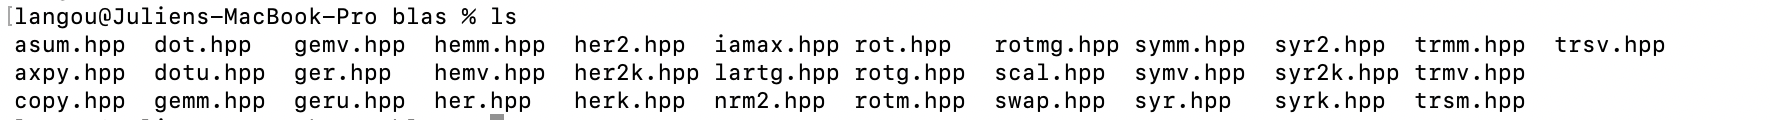
\includegraphics[width=\textwidth]{screenshots/tlapack-include-blas-ls.png}
\end{frame}

\begin{frame}{\tlapack (2/2)}
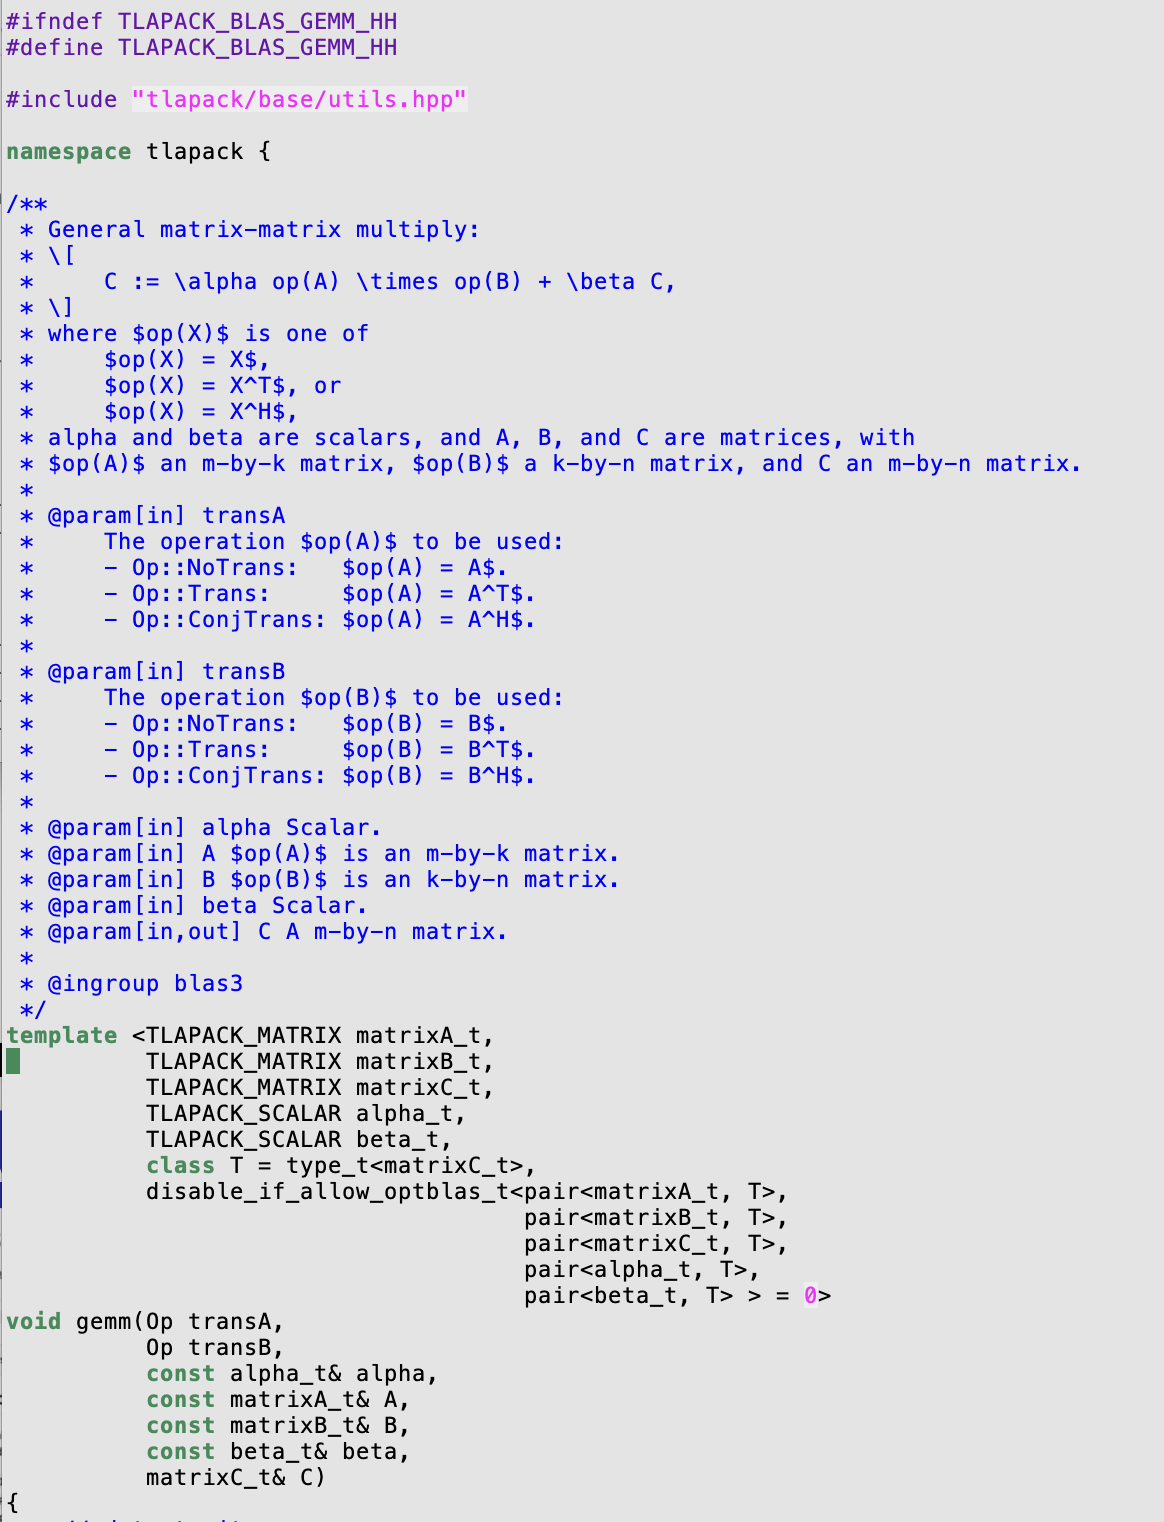
\includegraphics[height=\textheight]{screenshots/tlapack-gemm.png}
\end{frame}



\begin{frame}{We shall not forget LAPACK!}
We shall not forget LAPACK!
\end{frame}





% \begin{frame}{References}
% \printbibliography
% \end{frame}
\end{document}
